\chapter{}

\section{Diseño}

Hasta ahora, se ha mostrado de una forma muy abstracta, cómo interacciona el usuario con el \textit{bot}, por lo que vamos a abordar en primer lugar, cómo se puede hacer la interacción usuario-\textit{bot} antes de empezar a dar más forma al programa.

\subsection{Diseño de la interacción con el usuario}

\subsubsection{Chats grupales}
Conocer qué quiere un usuario por un chat grupal es fácil, ya que el \textit{bot} solo es invocado cuando recibe un mensaje en el formato \enquote*{/quiero\_hacer\_algo}\footnote{En realidad si pones como moderador a un bot de un chat puede recibir todos los mensajes de un chat}  es decir, que si alguien escribe \texttt{/temperatura Estambul} el bot recibe \texttt{/temperatura Estambul} pero si escriben \texttt{temperatura Roma} el \textit{bot} no recibe ningún mensaje. Esto hace que sea fácil para un usuario indicar al \textit{bot}  qué quiere por un chat grupal ya que solamente le hace falta conocer los comandos tipo \texttt{/comando xxx} que soporta el \textit{bot} y lo que hacen.
\subsubsection{Chats privados}

Más peliaguda es la interacción entre el usuario y el \textit{bot} en un chat privado  ya que, al contrario que en los CUs donde el actor era un usuario de un chat grupal, en la que toda interacción se reducía a un solo paso por parte del usuario en los CUs de los usuarios de los chats privados la realización de una acción requiere de varios pasos y utilizar el formato \texttt{/asignar\_solucion\_duda id\_duda 7 id\_respuesta 9 } queda sumamente críptico y poco amigable. Por todo lo anteriormente dicho se ha decidido utilizar los menús gráficos que nos proporciona Telegram:

\begin{figure}[H] %con el [H] le obligamos a situar aquí la figura
\centering
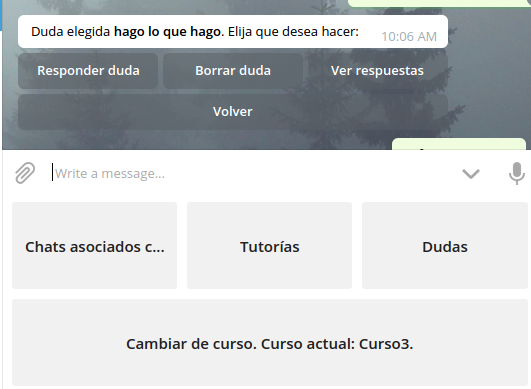
\includegraphics[scale=0.7]{imagenes/random/Screenshot_2017-08-21_13-09-40.png}  %el parámetro scale permite agrandar o achicar la imagen. En el nombre de archivo puede especificar directorios

\caption{Arriba menú tipo Inline, abajo menú tipo teclado}\label{figura10}
\end{figure}
Estos menús tienen la peculiaridad de que cuando un usuario pulsa una tecla  el bot recibe un mensaje tipo \enquote*{callback} (caso menús Inline) o de texto (menús tipo teclado) que identifica a la tecla pulsada dentro del menú.  Dicho lo cual, si se realiza un buen diseño de los menús, tanto el usuario como el bot pueden comprender perfectamente qué es lo que quiere el uno del otro.
\par
No se ha pensado en el uso de menús en los chats grupales porque pienso que generarían un ruido innecesario y que al ser interacciones \enquote*{de un solo paso} por parte del usuario son innecesarios.

\subsection{Diseño de la estructura}

Comenzamos a refinar el sistema para que éste empiece a estar lo suficientemente definido como para llevar a cabo su implementación. Hemos hablado brevemente del enrutamiento de mensajes en los CUs Reales y  en los diagramas anteriores hemos mostrado una clase \enquote*{pradobot} que es la encargada de conocer qué es lo que el usuario quiere y llevar a cabo las acciones pertinentes. Vamos a empezar a repartir las responsabilidades de dicha clase utilizando diferentes patrones de diseño. 
\subsubsection{Primera capa: controladores}

El bot es un programa que constantemente está escuchando por si Telegram le envía un nuevo mensaje y una vez recibido realiza una acción u otra.
Como hemos indicado en el apartado de diseño de interacción de usuario, la forma en que el bot se relaciona con un usuario entre un chat privado y uno grupal es muy diferente requiriendo la gestión de acciones que hacen uso de múltiples pasos mediante  menús para los usuarios de un chat privado ,mientras que las acciones que ejecutan los usuarios de los chats grupales solamente son de un paso y sin menús.

Esto nos lleva a aplicar el patrón \textbf{\enquote*{Controlador}} y distribuir las responsabilidades entre tres clases:
\begin{itemize}
\item \textbf{Mensajero}: su función es la de recibir mensajes, ver si proceden de un chat privado o grupal y transferir el mensaje a la clase responsable del manejo de mensajes procedentes de chats privados o a la de chats grupales.
\item \textbf{ManejadorMensajesChatsPrivados}: Recibe mensajes procedentes de un chat privado y lleva a cabo las siguientes funciones:
\begin{itemize}
\item Ver si el usuario que le habla está registrado en el sistema.
\item Controlar si el sistema ha acabado ya de procesar el último mensaje que le mandó el usuario.
\item Entregar el mensaje que le envía el usuario a una capa inferior para que ésta lleve a cabo una acción con el mensaje.
\end{itemize}
Esta clase no tiene la responsabilidad de ver qué se hace con el mensaje sino que lo transfiere a otra clase para que ésta lo procese.
\item \textbf{ManejadorMensajesChatsGrupales}: Recibe mensajes procedentes de un chat grupal. Sus funciones a destacar son:
\begin{itemize}
\item Controlar si los mensajes proceden de chats asociados a cursos del sistema.
\item Llevar a cabo el procesamiento del mensaje, lo cual desencadena en una acción.
\end{itemize}
Como  esta clase es la que conoce qué chat corresponde a qué curso y las interacciones con los chats grupales son tan básicas, se le ha asignado también la responsabilidad de ejecutar lo que quiere el usuario en el mensaje.
\end{itemize}

Podemos ver el funcionamiento de esta primera capa en las siguientes capturas:
\begin{figure}[H] %con el [H] le obligamos a situar aquí la figura
\centering
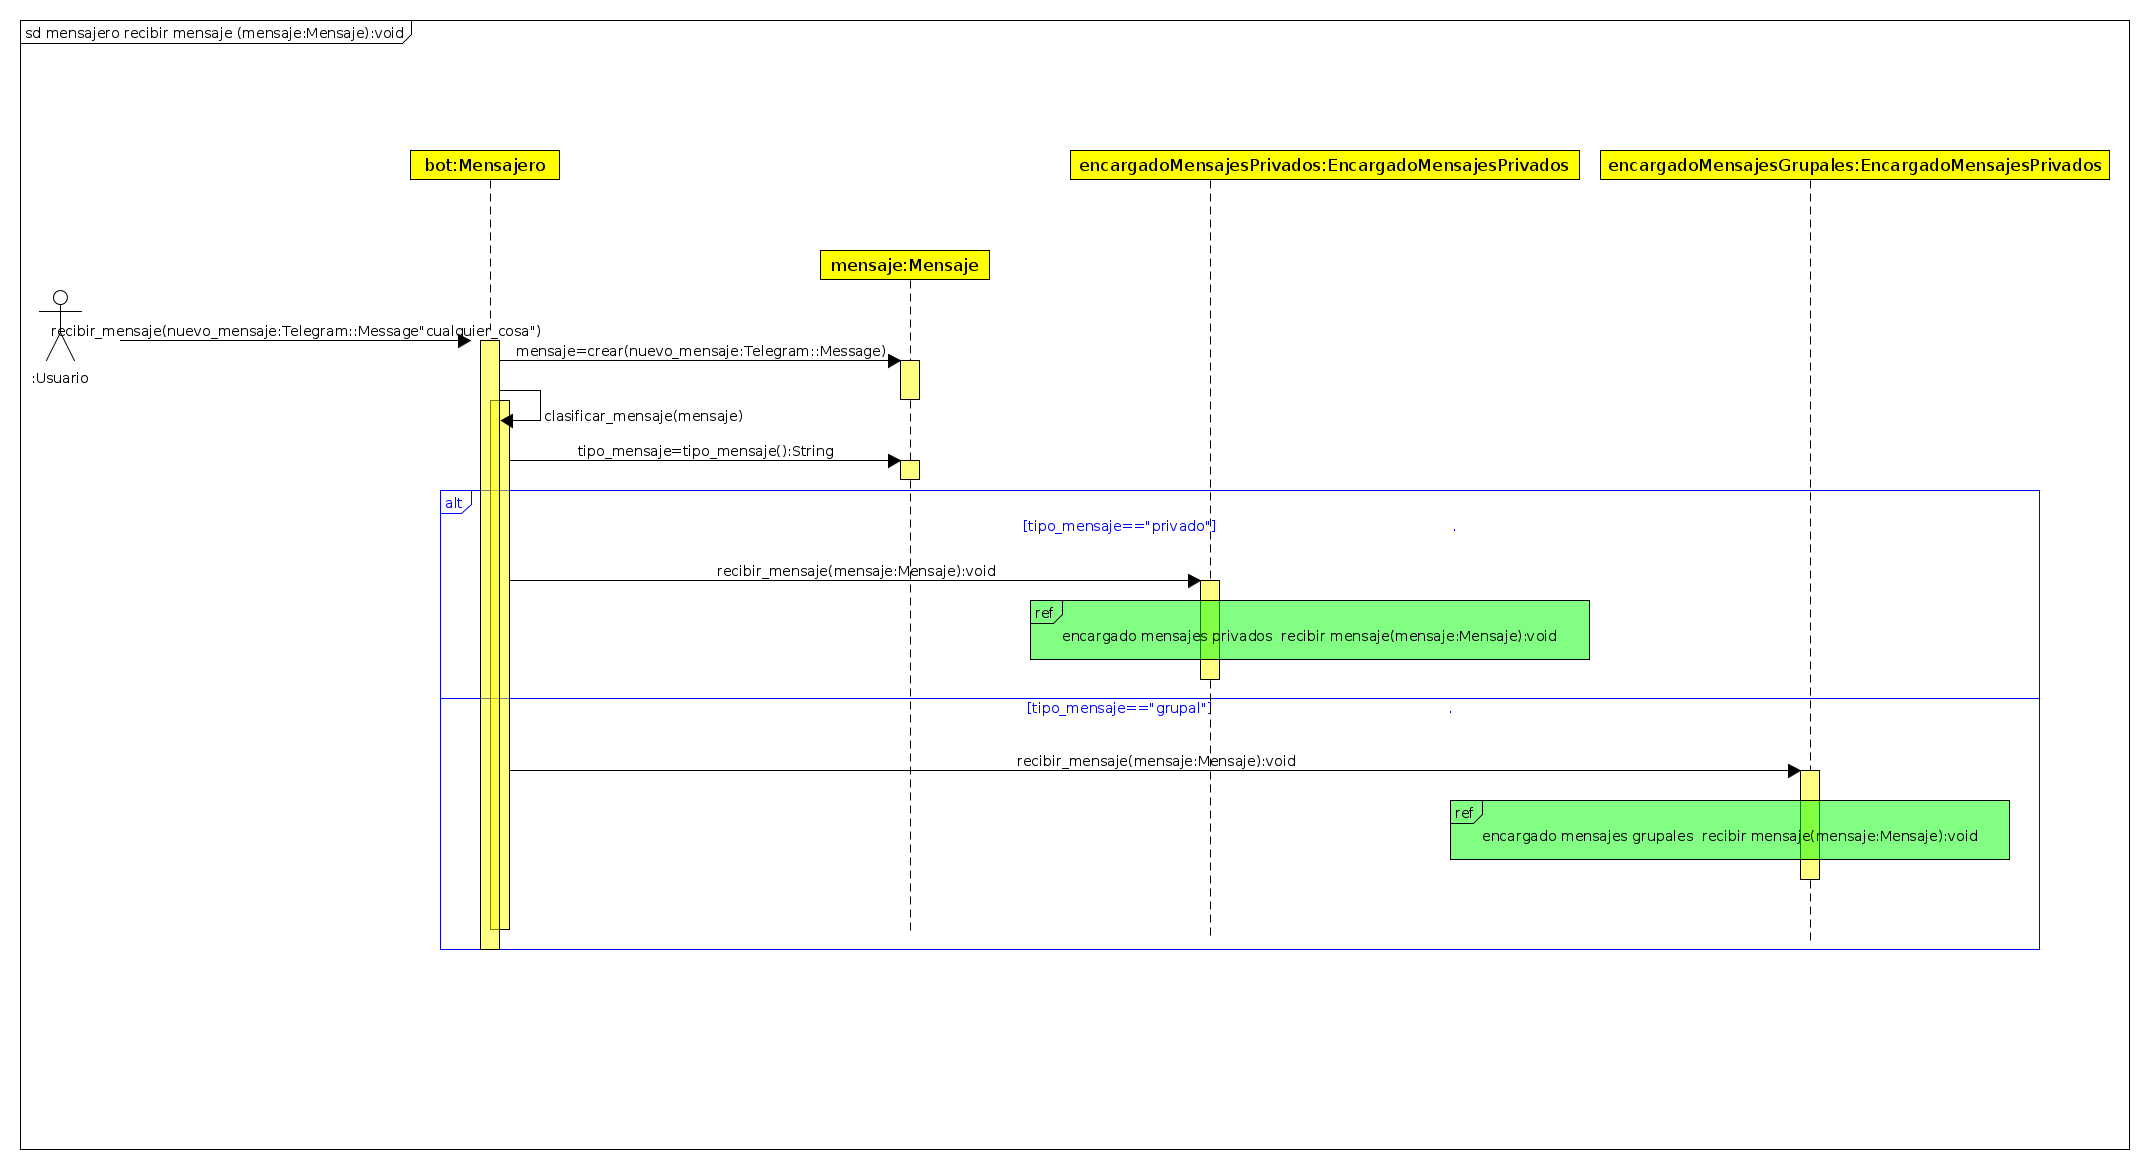
\includegraphics[scale=0.2]{imagenes/diagramas/secuencia/grandes/nuevo_mensaje.png}  %el parámetro scale permite agrandar o achicar la imagen. En el nombre de archivo puede especificar directorios

\caption{Diagrama secuencia recibir\_mensaje clase  Mensajero: el bot recibe un nuevo mensaje}\label{figura220}
\end{figure}

He preferido mostrar el funcionamiento de como opera el ManejadorMensajesPrivados debido a que es bastante más complejo que el de chats grupales:


\begin{figure}[H] %con el [H] le obligamos a situar aquí la figura
\centering
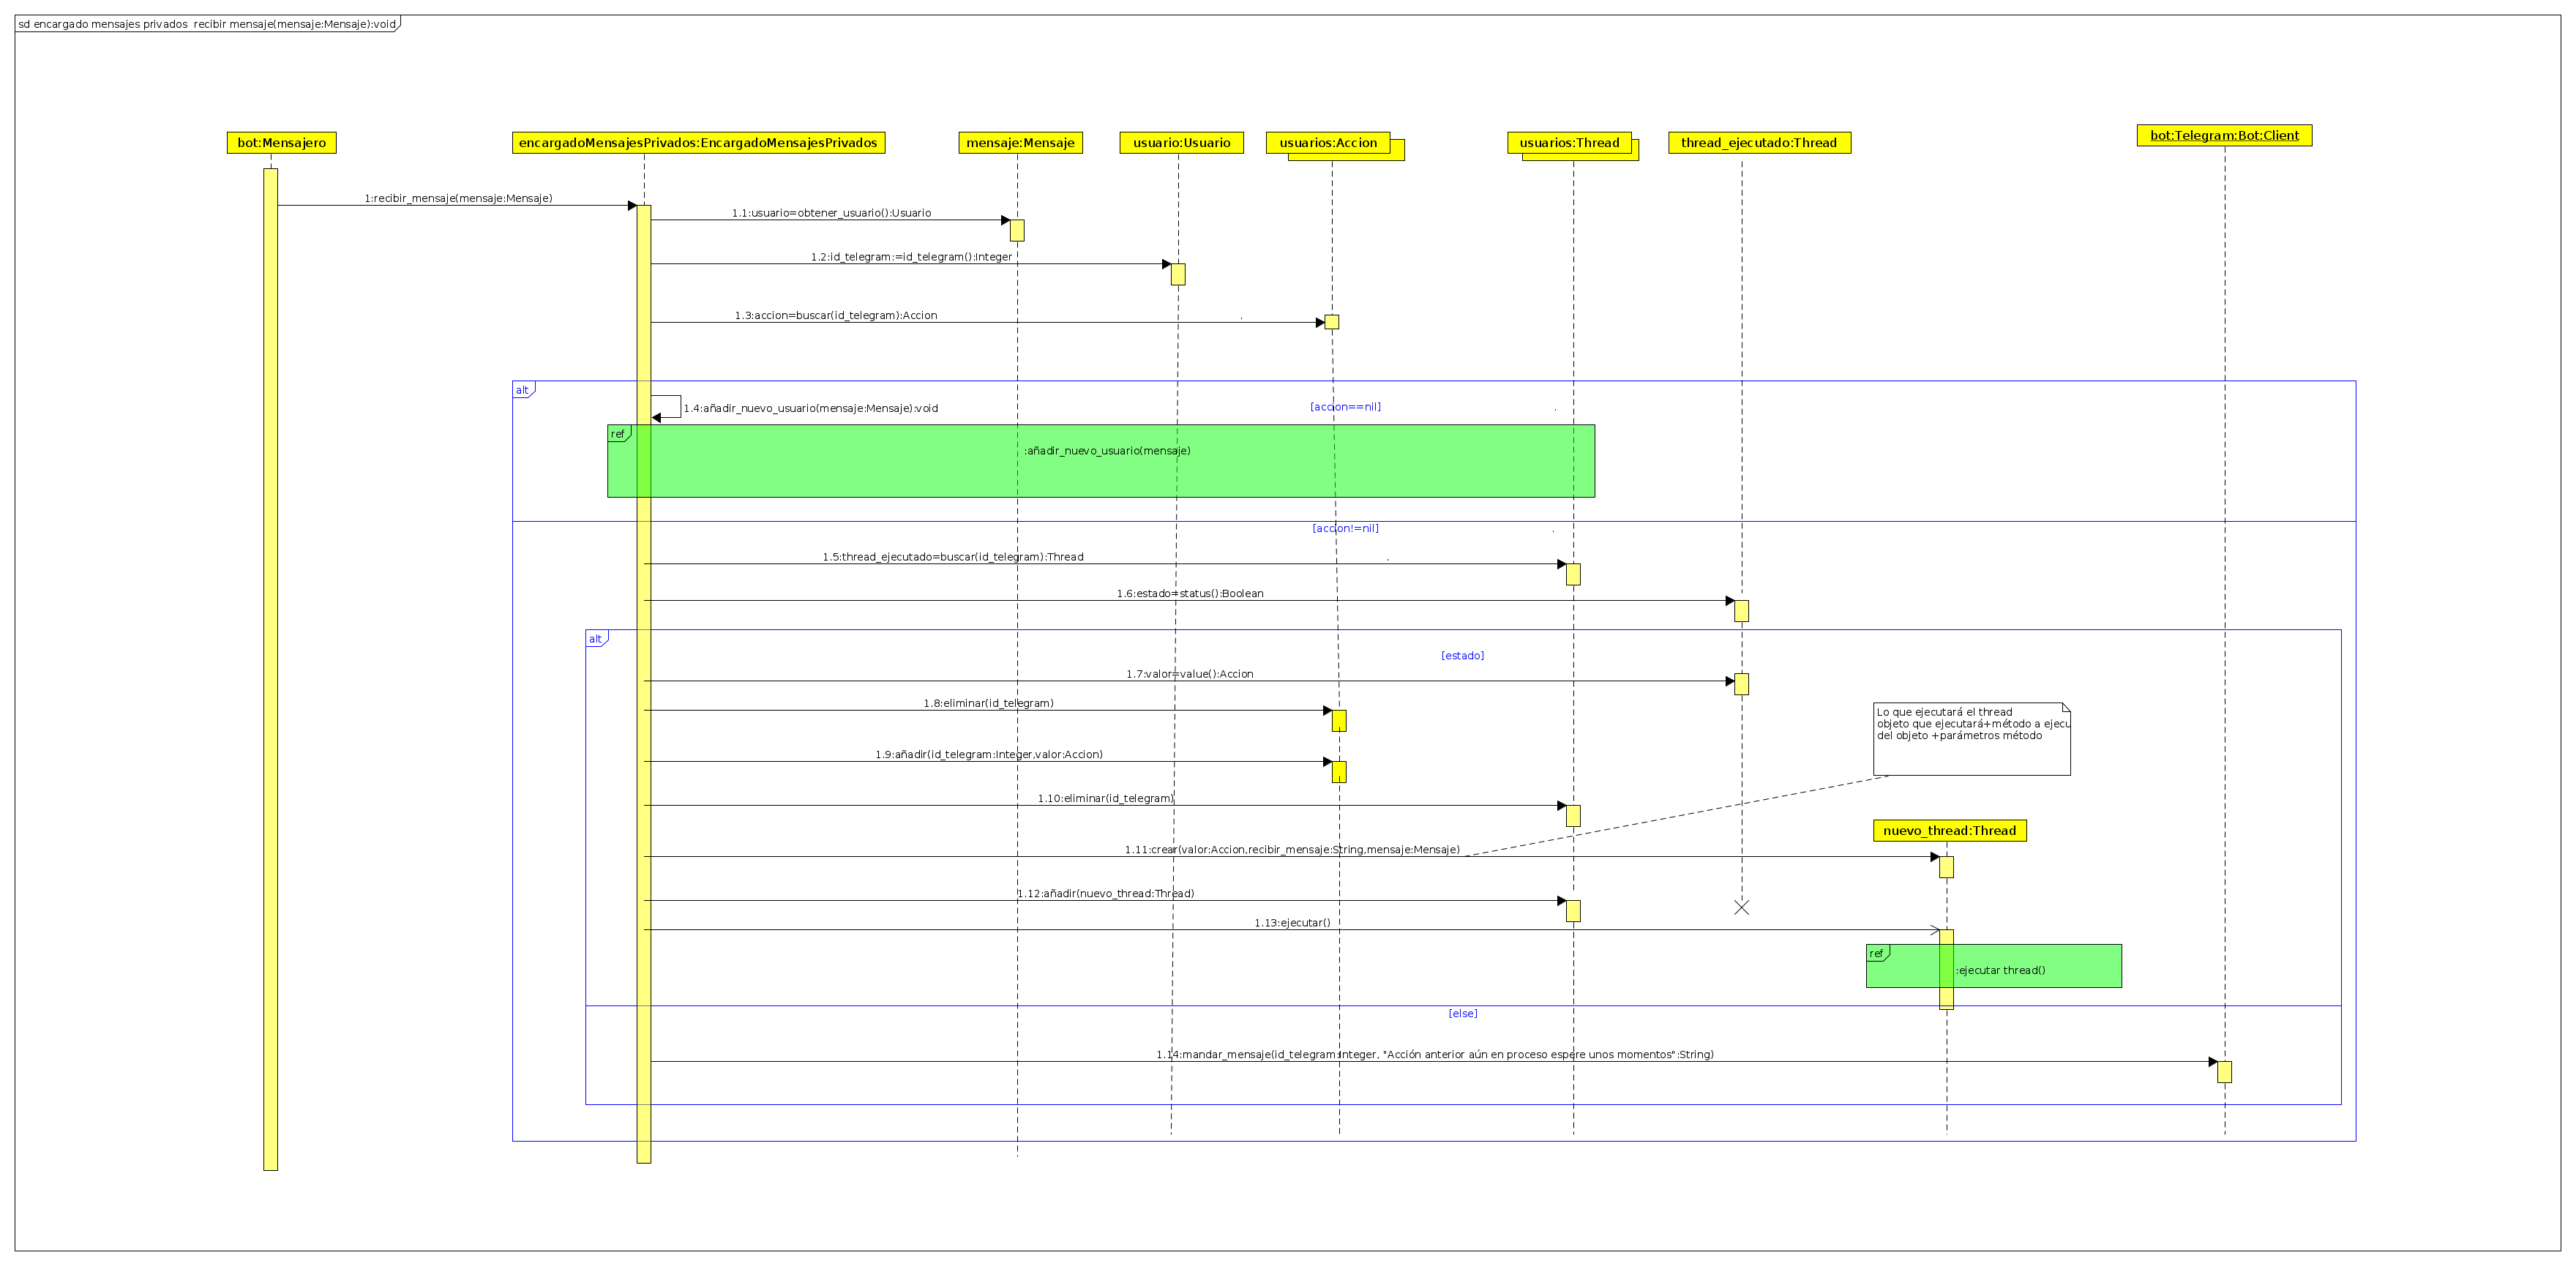
\includegraphics[scale=0.12]{imagenes/diagramas/secuencia/grandes/clasificar_mensaje_comprimido.png}  %el parámetro scale permite agrandar o achicar la imagen. En el nombre de archivo puede especificar directorios

\caption{Diagrama secuencia recibir\_mensaje clase  ManejadorMensajesChatsPrivados}\label{figura221}
\end{figure}




\begin{figure}[H] %con el [H] le obligamos a situar aquí la figura
\centering
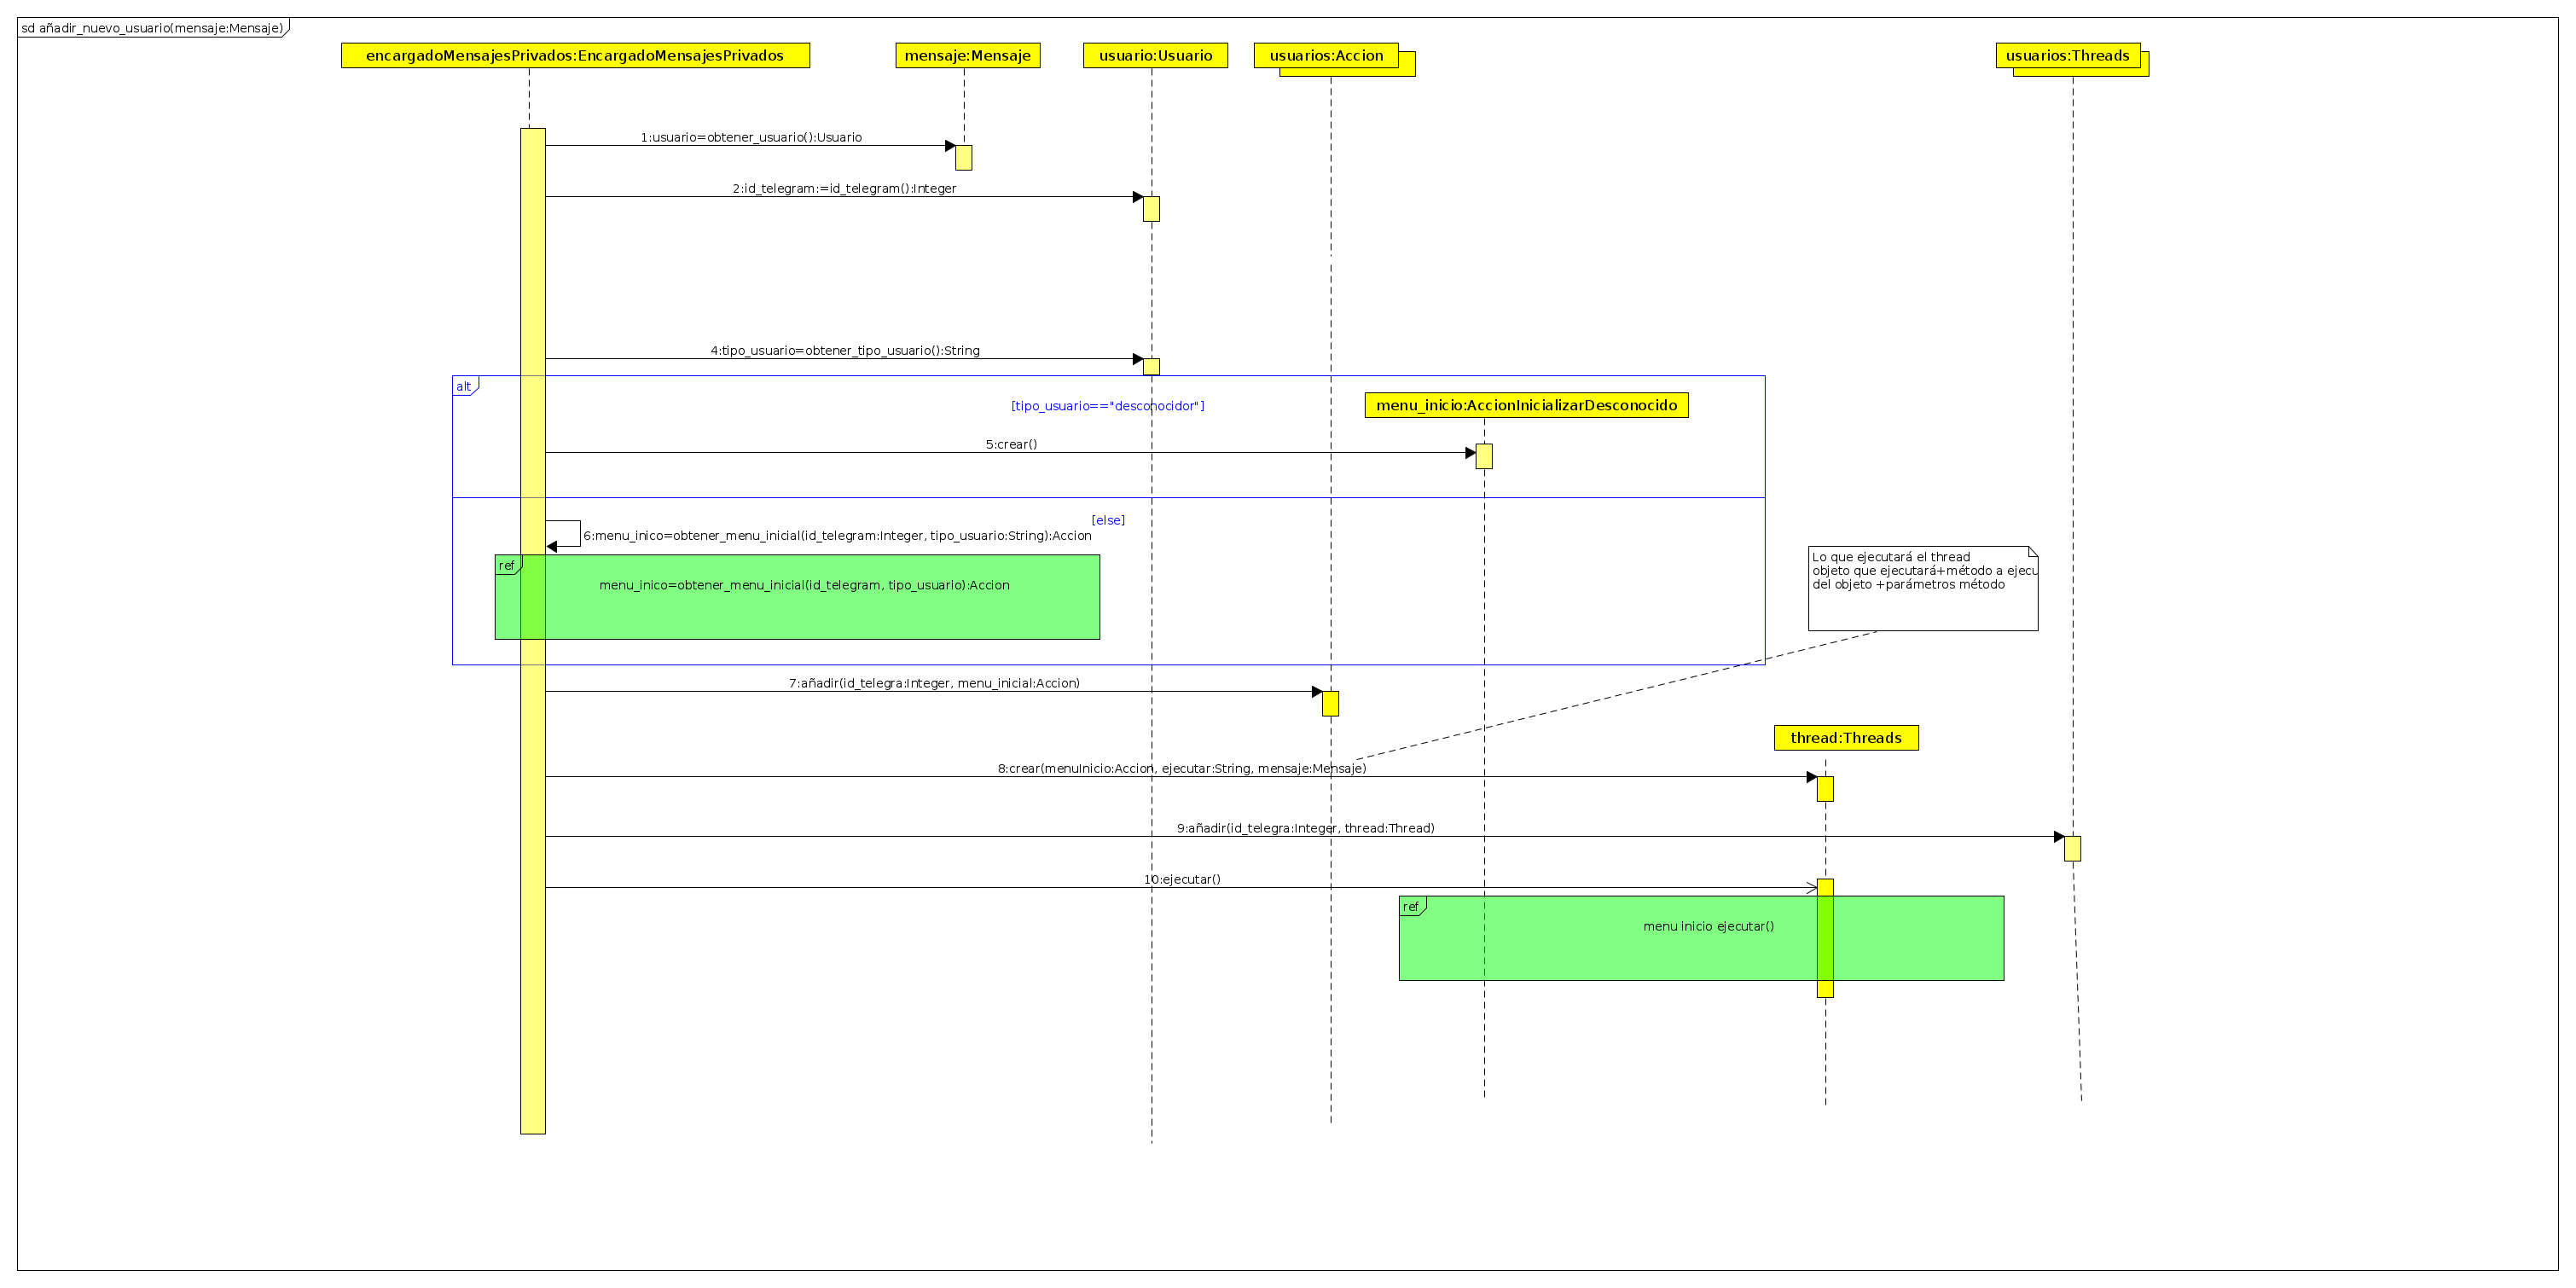
\includegraphics[scale=0.14]{imagenes/diagramas/secuencia/grandes/anadir_nuevo_usuario.png}  %el parámetro scale permite agrandar o achicar la imagen. En el nombre de archivo puede especificar directorios

\caption{Diagrama secuencia añadir\_nuevo\_usuario clase  ManejadorMensajesChatsPrivados}\label{figura222}
\end{figure}


\begin{figure}[H] %con el [H] le obligamos a situar aquí la figura
\centering
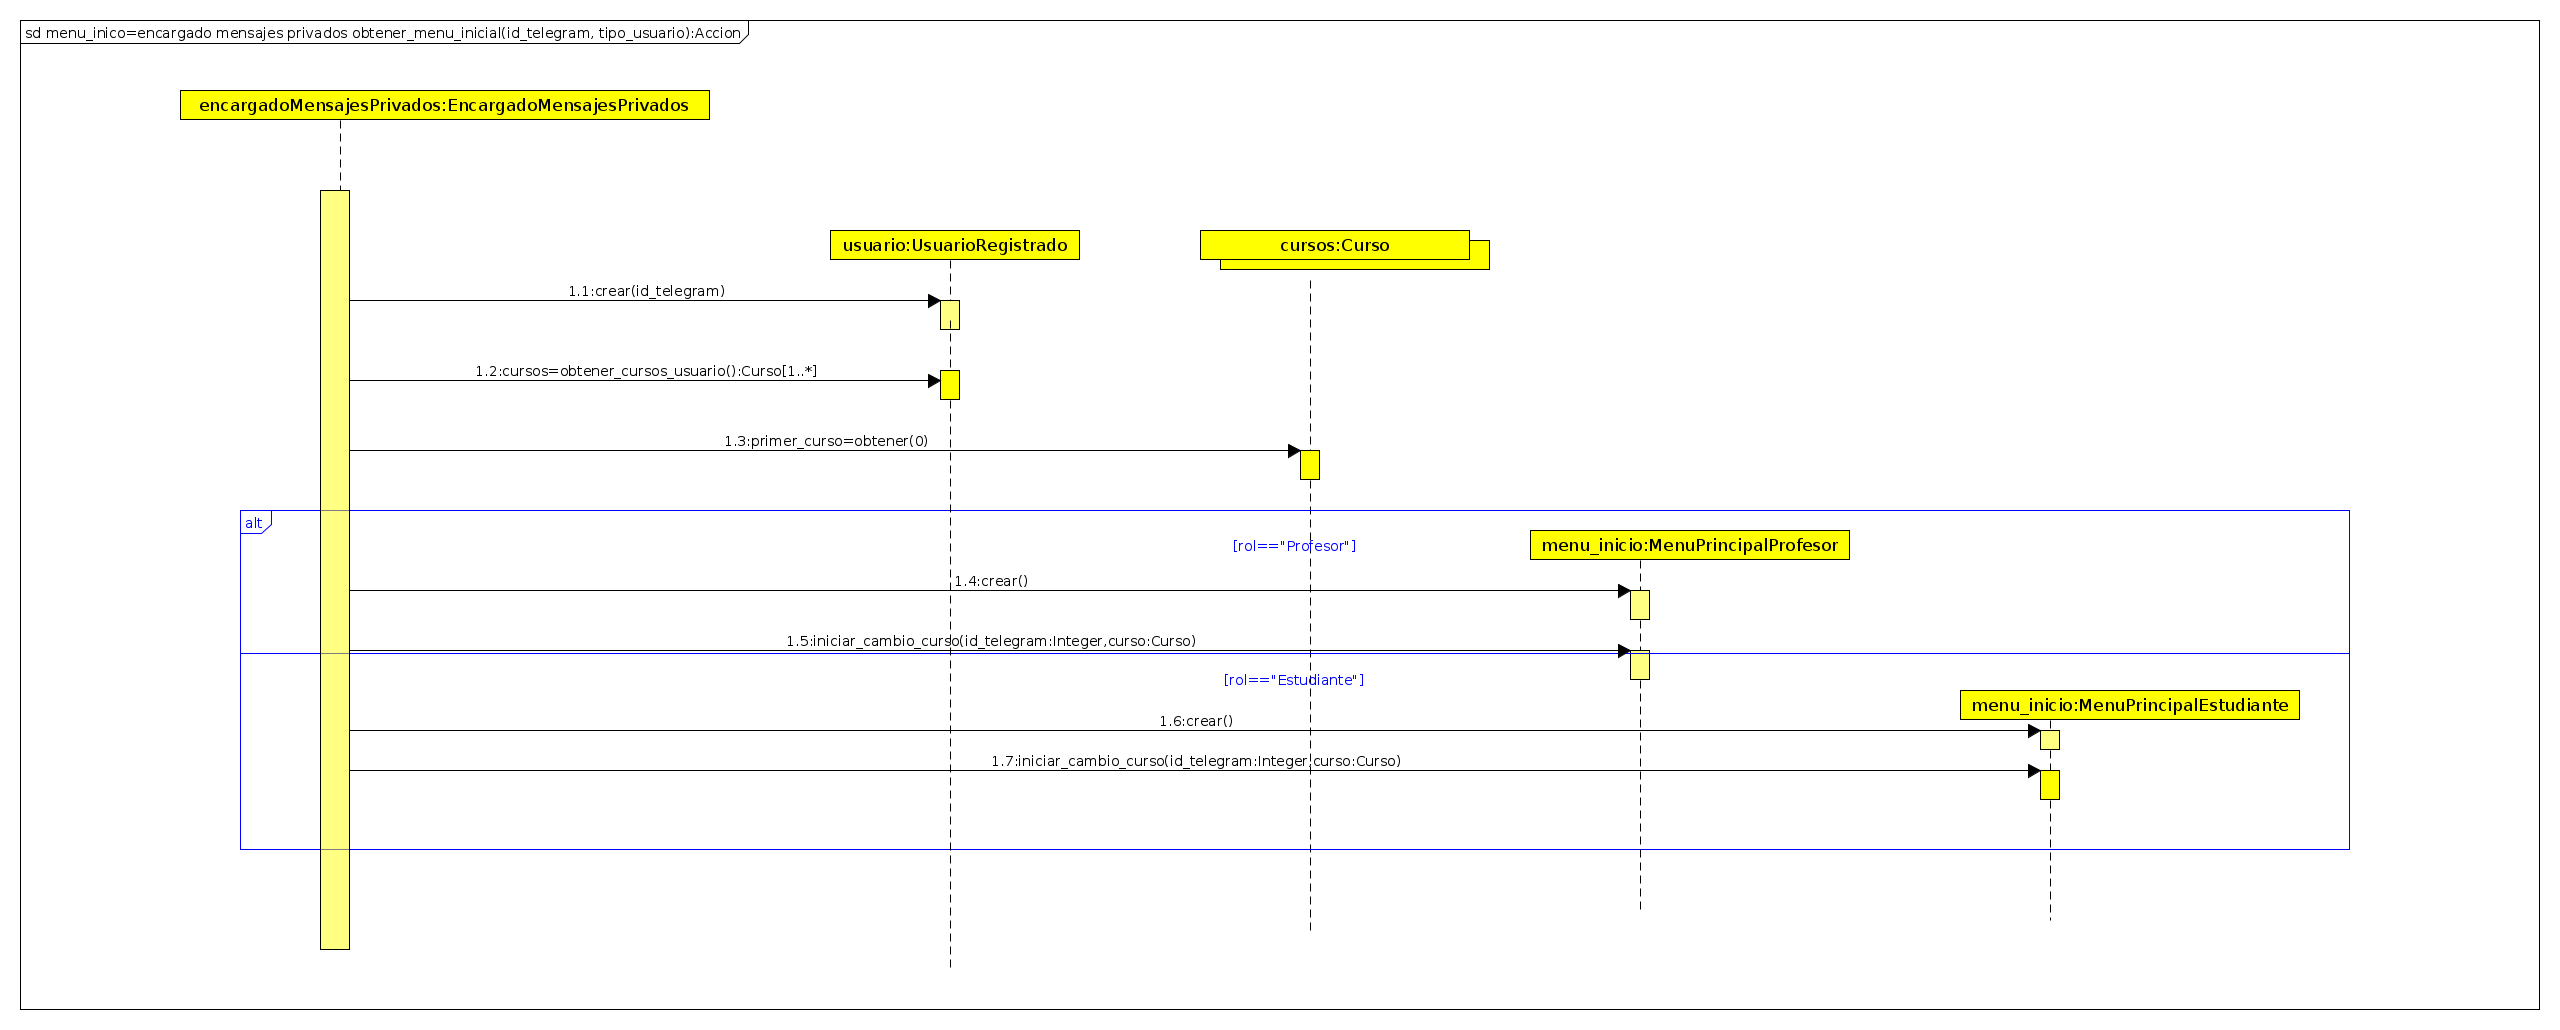
\includegraphics[scale=0.16]{imagenes/diagramas/secuencia/grandes/obtener_menu_inicio.png}  %el parámetro scale permite agrandar o achicar la imagen. En el nombre de archivo puede especificar directorios

\caption{Diagrama secuencia obtener\_menu\_inicio clase  ManejadorMensajesChatsPrivados}\label{figura223}
\end{figure}

\begin{figure}[H] %con el [H] le obligamos a situar aquí la figura
\centering
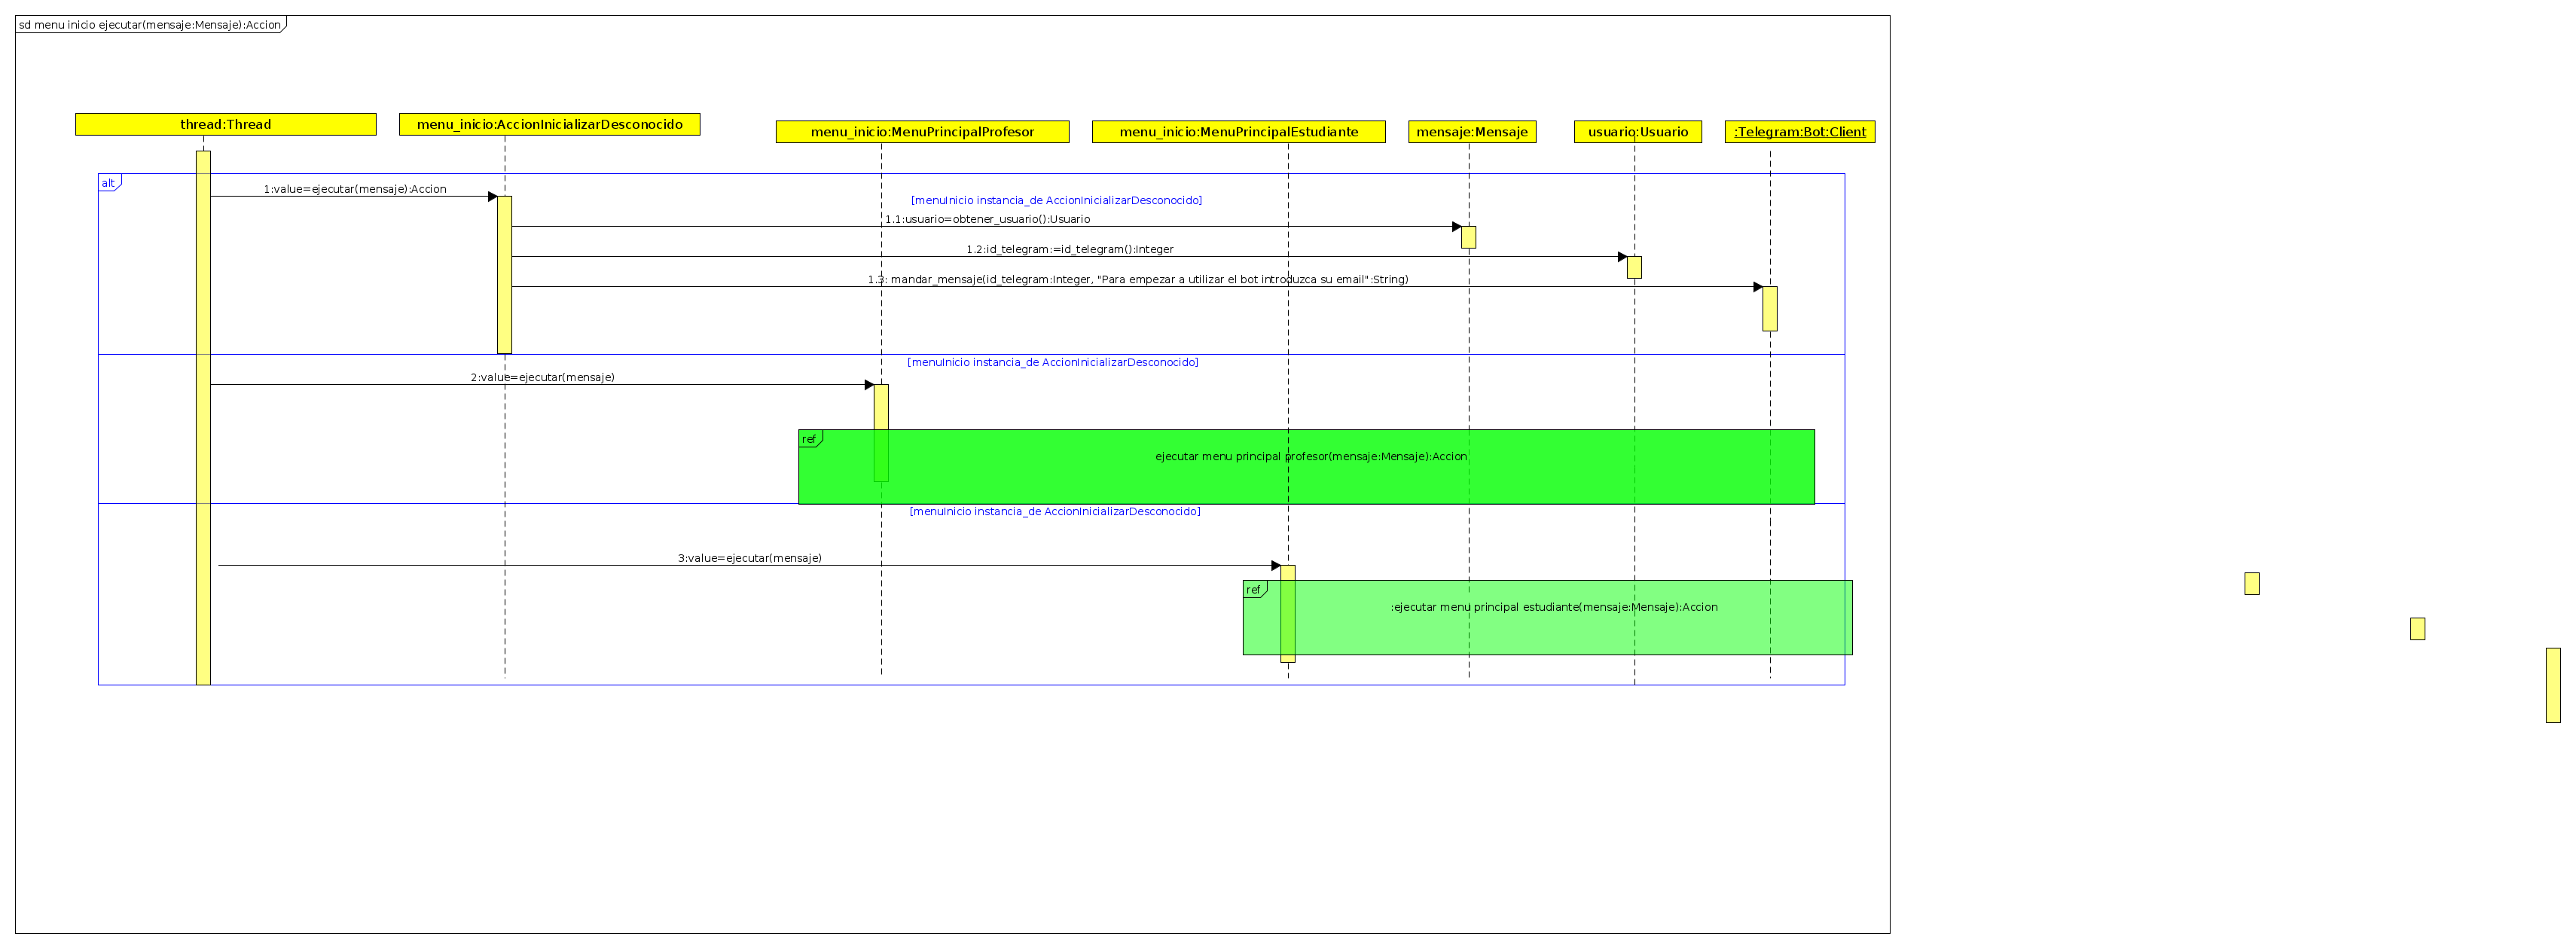
\includegraphics[scale=0.16]{imagenes/diagramas/secuencia/grandes/menu_inicio_ejecutar.png}  %el parámetro scale permite agrandar o achicar la imagen. En el nombre de archivo puede especificar directorios

\caption{Diagrama secuencia ejecutar\_menu\_inicio clase  ManejadorMensajesChatsPrivados}\label{figura227}
\end{figure}

En la siguiente captura se puede apreciar el polimorfismo. Explciaremos su uso en el programa en la siguiente sección.

\begin{figure}[H] %con el [H] le obligamos a situar aquí la figura
\centering
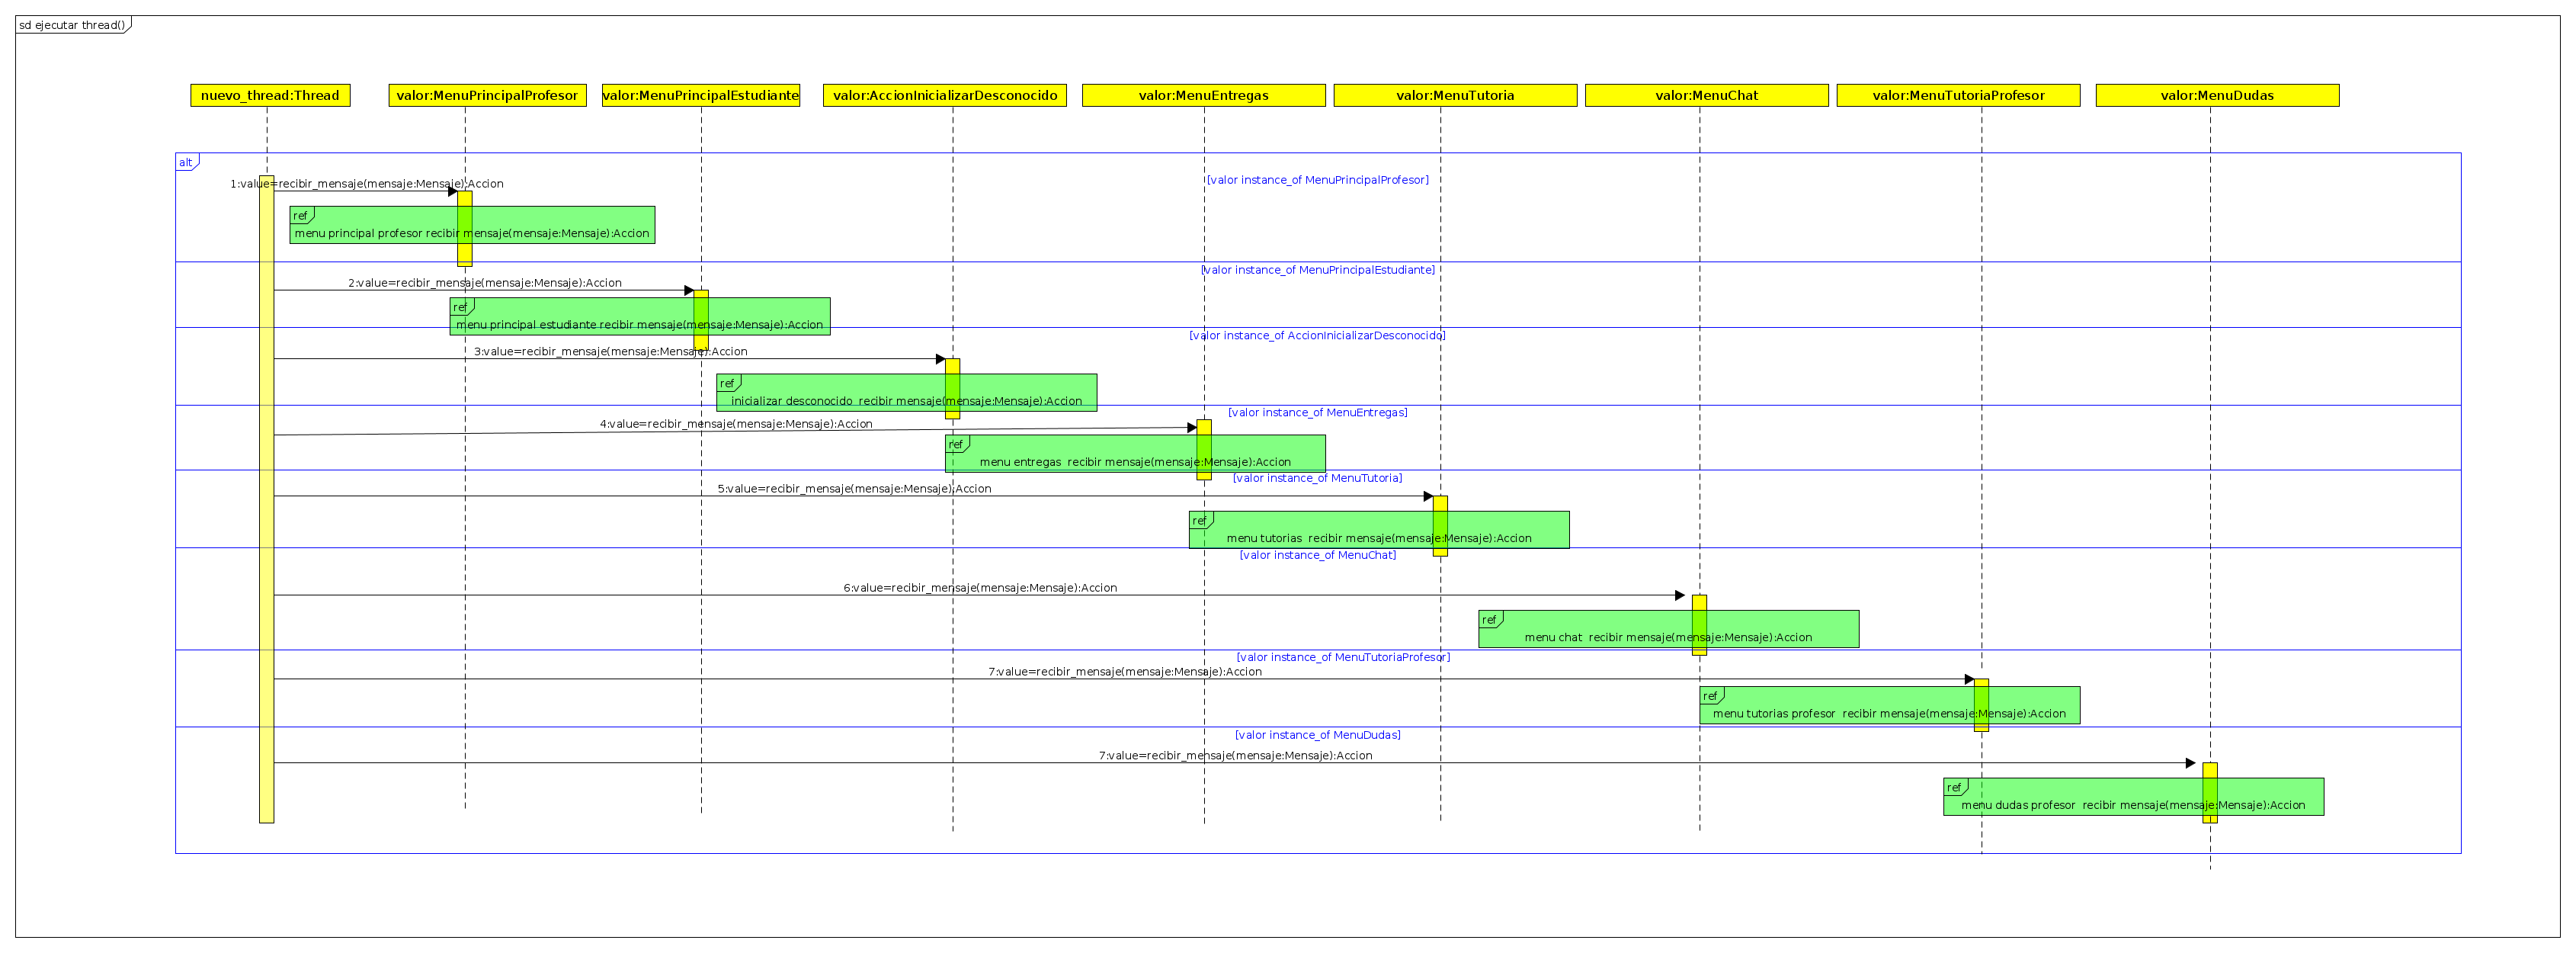
\includegraphics[scale=0.13]{imagenes/diagramas/secuencia/grandes/ejecutar_thread.png}  %el parámetro scale permite agrandar o achicar la imagen. En el nombre de archivo puede especificar directorios

\caption{Diagrama secuencia muestra ejecución thread iniciado por ManejadorMensajesChatsPrivados }\label{figura223}
\end{figure}
\subsubsection*{Segunda capa: menús}


\textbf{ManejadorMensajesChatsPrivados} le pasa el mensaje a otra clase que es la encargada de ver qué quiere el usuario con el mensaje. 
 Debido al diseño mediante menús que se ha decidido hacer  para interaccionar con el usuario, la clase que realmente sabe qué es lo que quiere hacer el usuario con su mensaje es aquella que controla al menú que está viendo el usuario ya que ésta es la que conoce las opciones contenidas en el menú. El mensaje que recibe un menú puede indicar tres cosas:
\begin{itemize}
\item Selección de una nueva opción del menú.
\item Indicar que se quiere cambiar de menú.
\item El mensaje no está destinado al menú sino a la última opción que pulsó el usuario en el menú.
\end{itemize} 
 
 El procesamiento de un mensaje por parte de una clase menú siempre devuelve otra clase menú que será la que reciba el proximo mensaje de ManejadorMensajesChatsPrivados. Puede devolverse a ella misma o a su menú padre. He aquí el \textbf{Polimorfismo}.
 La jerarquía de menús puede descomponerse en:
 
 \begin{itemize}
 \item MenuPrincipalEstudiante: El menú que vé un estudiante la primera vez que le manda un mensaje al bot. Contiene:
 \begin{itemize}
 \item MenuTutorias
 \item MenuEntregas
 \item MenuDudas
 \end{itemize}
 \item MenuPrincipalProfesor: Igual que el menú anterior pero para el profesor. Contiene:
 \begin{itemize}
 \item MenuTutoriasProfesor
 \item MenuChatTelegram
 \item MenuDudas
 \end{itemize}
\item MenuTutoriasProfesor: Contiene las opciones:
\begin{itemize}
\item Ver cola de tutorías
\item Crear tutoría
\item Borrar tutoría.
\end{itemize}
\item MenuChatTelegram: Contiene las opciones:
\begin{itemize}
\item Asociar curso a chat.
\end{itemize}
\item MenuTutorias: Permite al estudiante elegir entre:
\begin{itemize}
\item Solicitar asistencia tutoría.
\item Ver estado de sus solicitudes.
\end{itemize}
\item MenuEntregas: Permite al estudiante:
\begin{itemize}
\item Obtener información de próximas entregas.
\item Ver calificaciones.
\end{itemize}
\item MenuDudas: contiene las opciones: 
\begin{itemize}
\item Crear duda.
\item Opción que permite: 
\begin{itemize}
\item Ver dudas con solución.
\item Ver dudas sin solución.
\item Ver dudas del usuario.
\item Ver respuestas dudas.
\item Seleccionar una respuesta como solución a duda.
\item Borrar duda.
\end{itemize}
 \end{itemize}
\end{itemize}

La jerarquía de menús se ha diseñado con especial énfasis en que las acciones que realizan algo similar estén contenidas en el mismo menú. Aquellas opciones que permiten más de una opción han sido anidadas así para evitar la repetición de acciones por parte de un usuario. Ejemplo:\par
Si un usuario selecciona una duda se le muestre que puede borrar la duda, ver sus respuestas, asignarle una solución... y no al revés, es decir,  tener un menú con la opción borrar duda, ver respuestas, asignarle solución y que nada más pulsar cualquiera de ellas te solicite que elijas la duda.
\par
Todos los menús, además, contienen la opción de cambiar de curso y  la de volver al menú anterior (menos los menús principales ya que no tienen menú anterior).





\subsubsection{Tercera capa: opciones de menús}


Cada opción de un menú está representada por una clase, que es la que conoce los pasos que tiene que realizar un usuario para llevar a cabo la acción que representa, así como de mediar entre el usuario y los \enquote*{objetos} que intervienen en esa acción. Recibe los mensajes procedentes del menú que la contiene y de ellos extrae la información que necesita.


\subsubsection{Cuarta capa: contenedores de datos}
El objetivo de las clases de esta capa es la de hacer de árbitro entre los datos ( Moodle y la base de datos) y el resto del sistema. Son las únicas que utilizan la API de Moodle cuando es necesario y hacen llamadas a la base de datos cuando se les solicita un dato de la clase que simbolizan (ejemplo: dudas creadas por un usuario).

Para ilustrar las interacciones entre la tercera y cuarta capas podemos ver el siguiente diagrama de comunicación de la opción solicitar tutoría que recibe mensaje de menú MenuTutorias:


\begin{figure}[H] %con el [H] le obligamos a situar aquí la figura
\centering
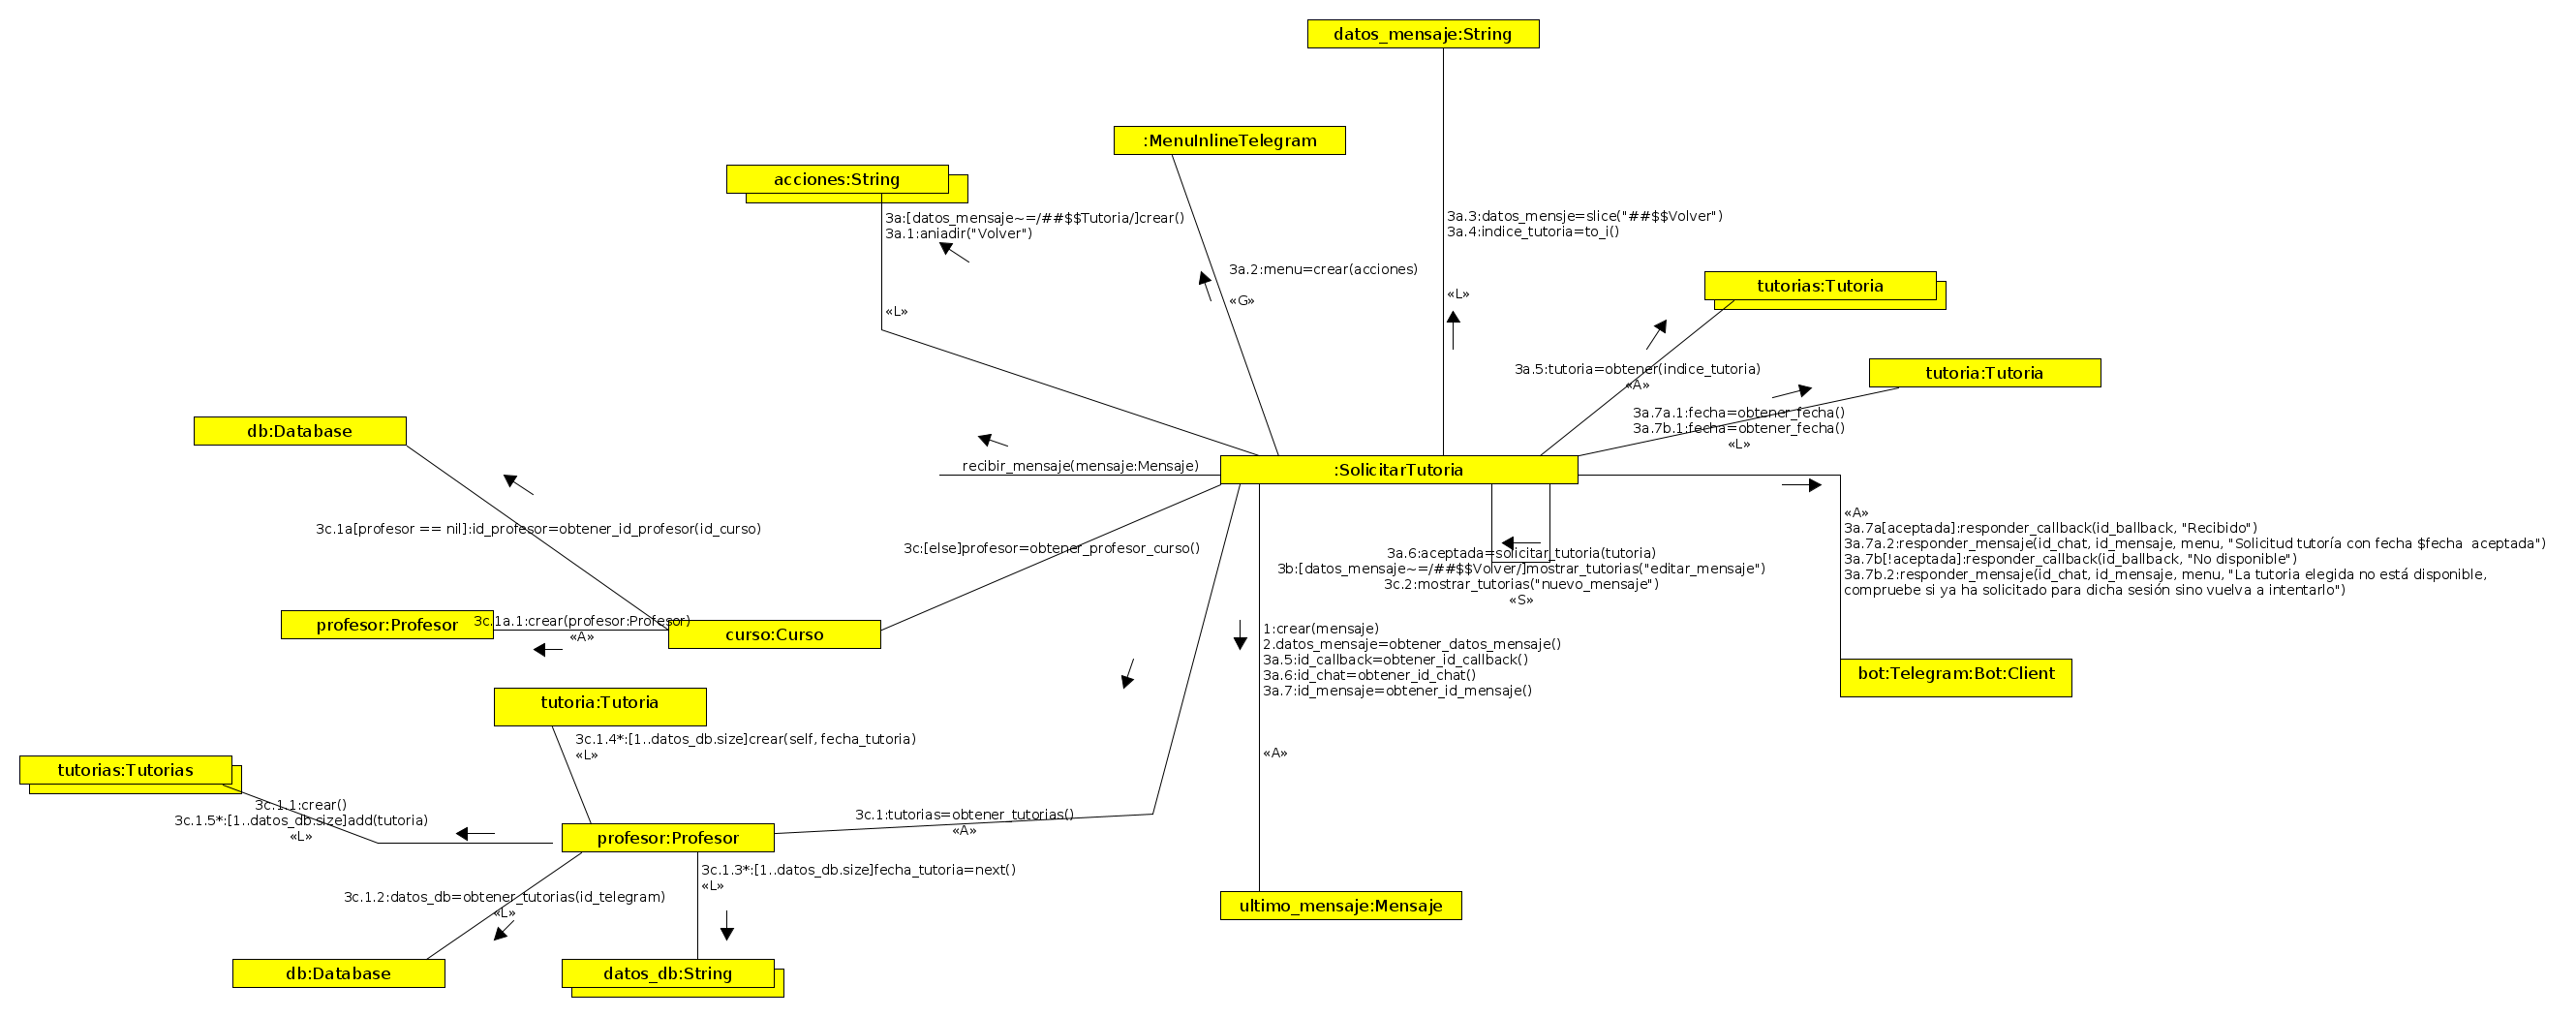
\includegraphics[scale=0.18]{imagenes/diagramas/comunicacion/solicitar_tutoria_recibir_mensaje.png}  %el parámetro scale permite agrandar o achicar la imagen. En el nombre de archivo puede especificar directorios

\caption{Diagrama comunicación recibir\_mensaje clase  SolicitarTutoria}\label{figura110}
\end{figure}

En el diagrama se puede observar como la clase SolicitarTutoria crea y envía diferentes mensajes al usuario empleando para el contenido de estos información de las clases Profesor y Tutoría.


\begin{figure}[H] %con el [H] le obligamos a situar aquí la figura
\centering
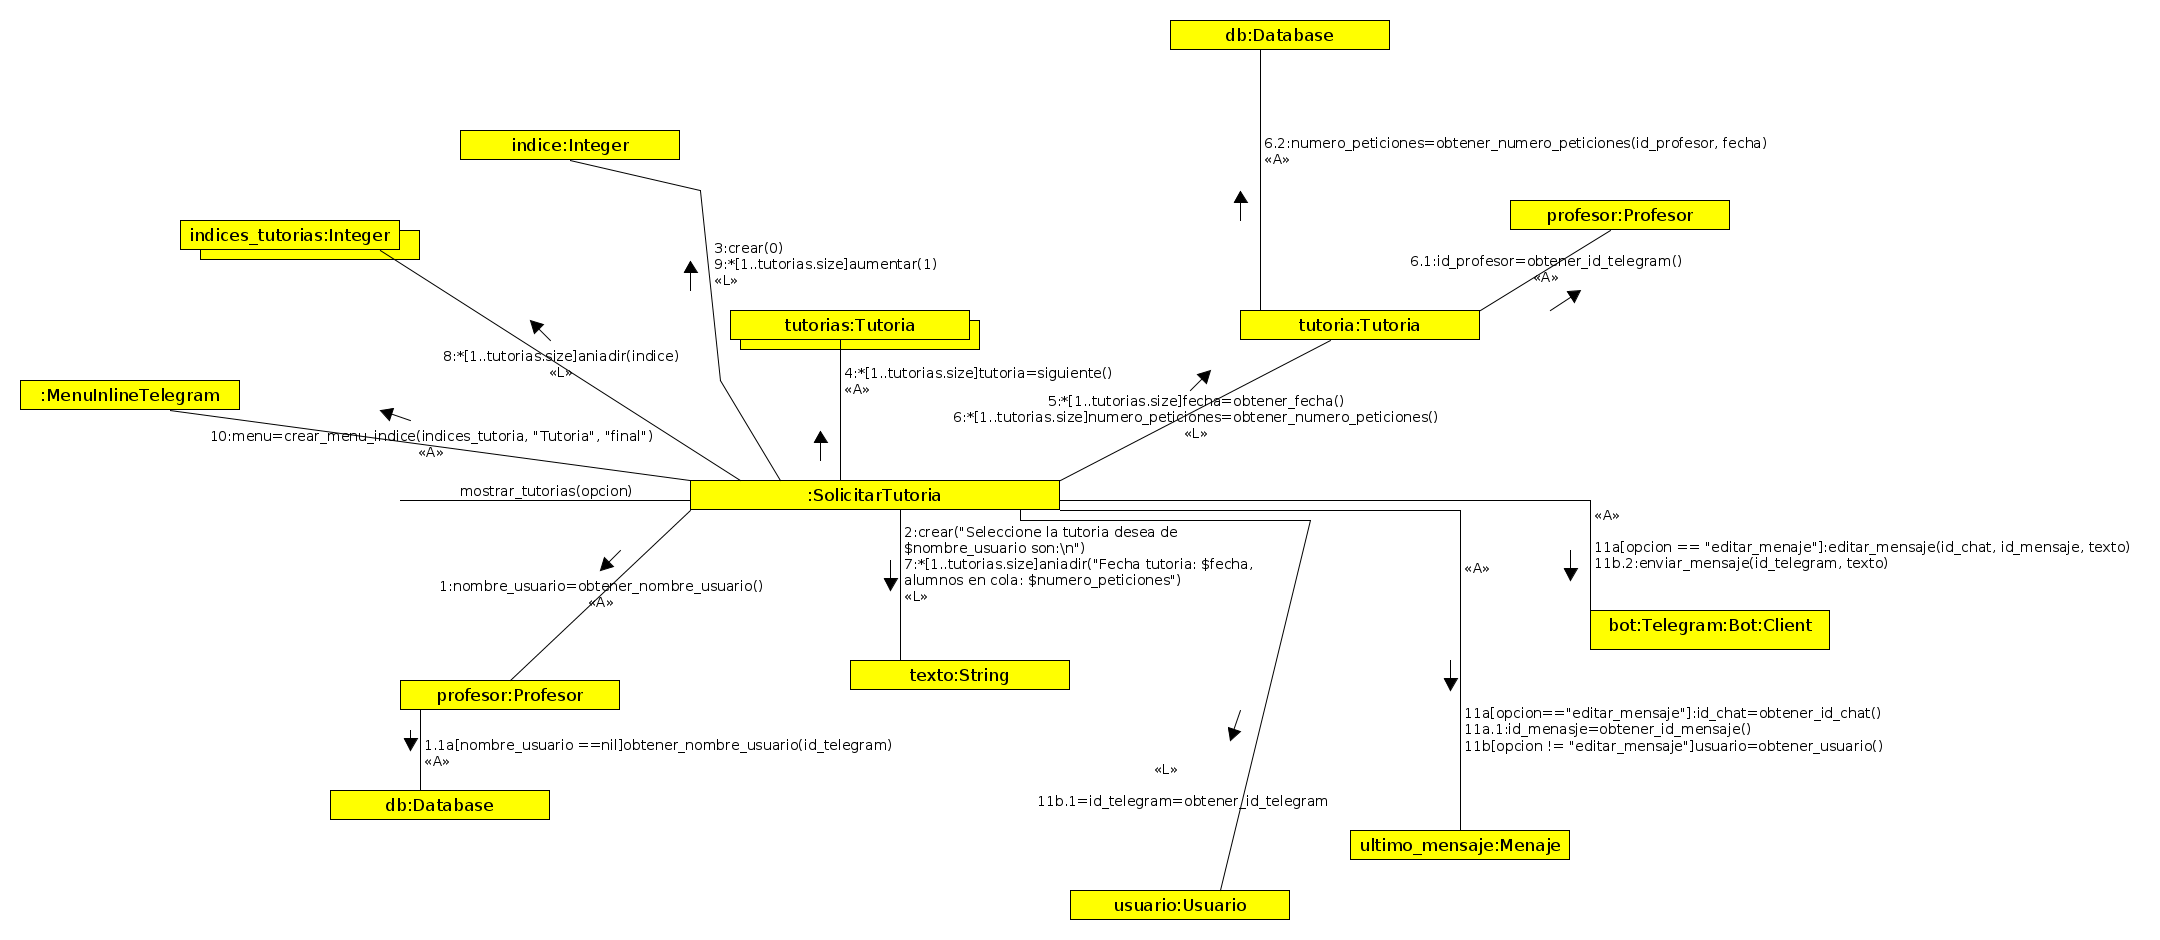
\includegraphics[scale=0.2]{imagenes/diagramas/comunicacion/mostrar_tutorias.png}  %el parámetro scale permite agrandar o achicar la imagen. En el nombre de archivo puede especificar directorios

\caption{Diagrama comunicación mostrar\_tutorías clase  SolicitarTutoria}\label{figura111}
\end{figure}


\begin{figure}[H] %con el [H] le obligamos a situar aquí la figura
\centering
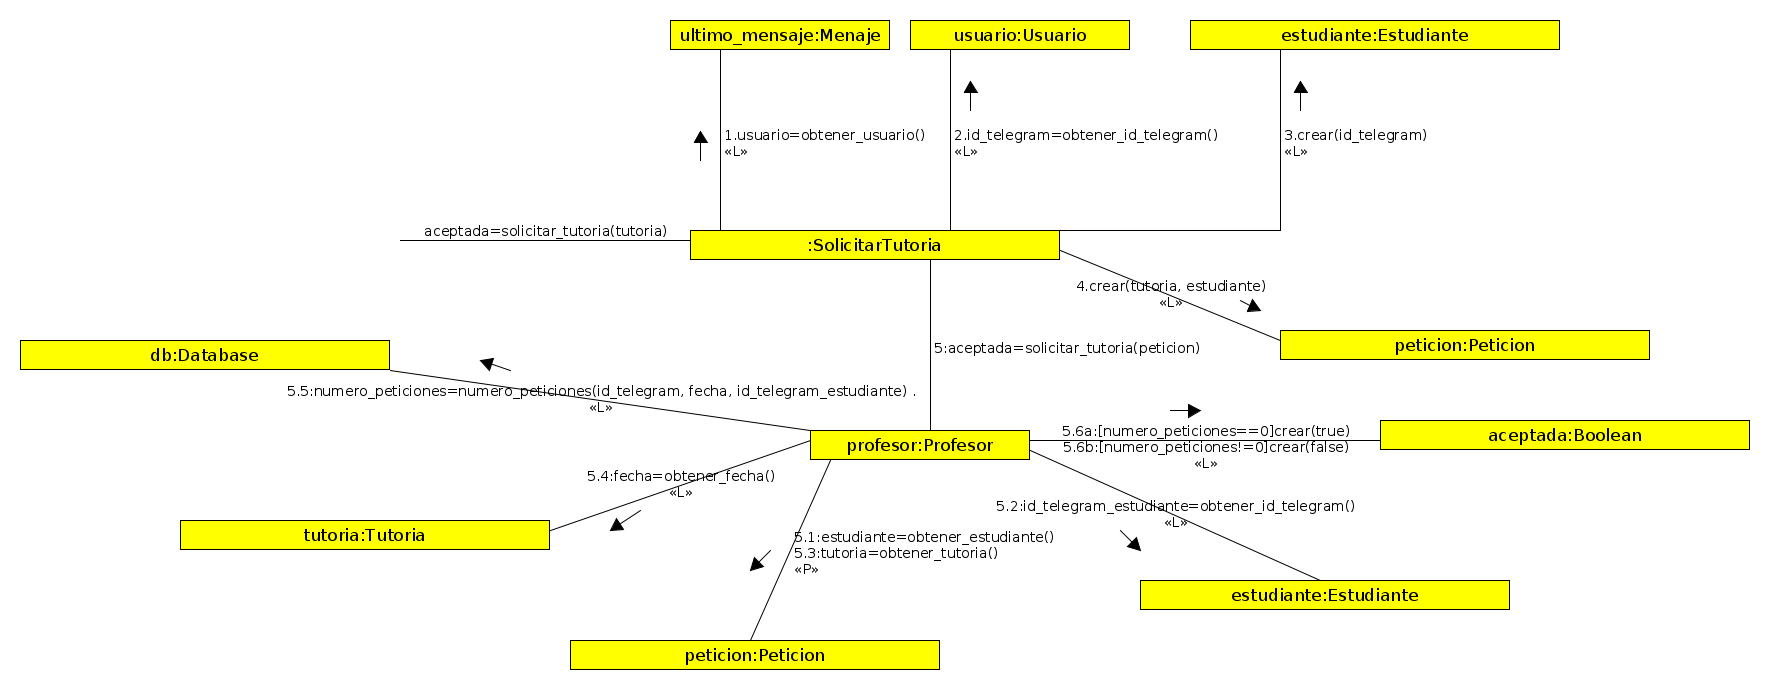
\includegraphics[scale=0.2]{imagenes/diagramas/comunicacion/solicitar_tutoria_tutoria.png}  %el parámetro scale permite agrandar o achicar la imagen. En el nombre de archivo puede especificar directorios

\caption{Diagrama comunicación solicitar\_tutoria clase  SolicitarTutoria}\label{figura112}
\end{figure}

El diagrama de clases obtenido al final para la aplicación sale demasiado grande para que sea fácilmente visible en el pdf. Se puede encontrar dentro de la carpeta diagramas con el nombre diagrama\_clases.png.

 \begin{figure}[H] %con el [H] le obligamos a situar aquí la figura
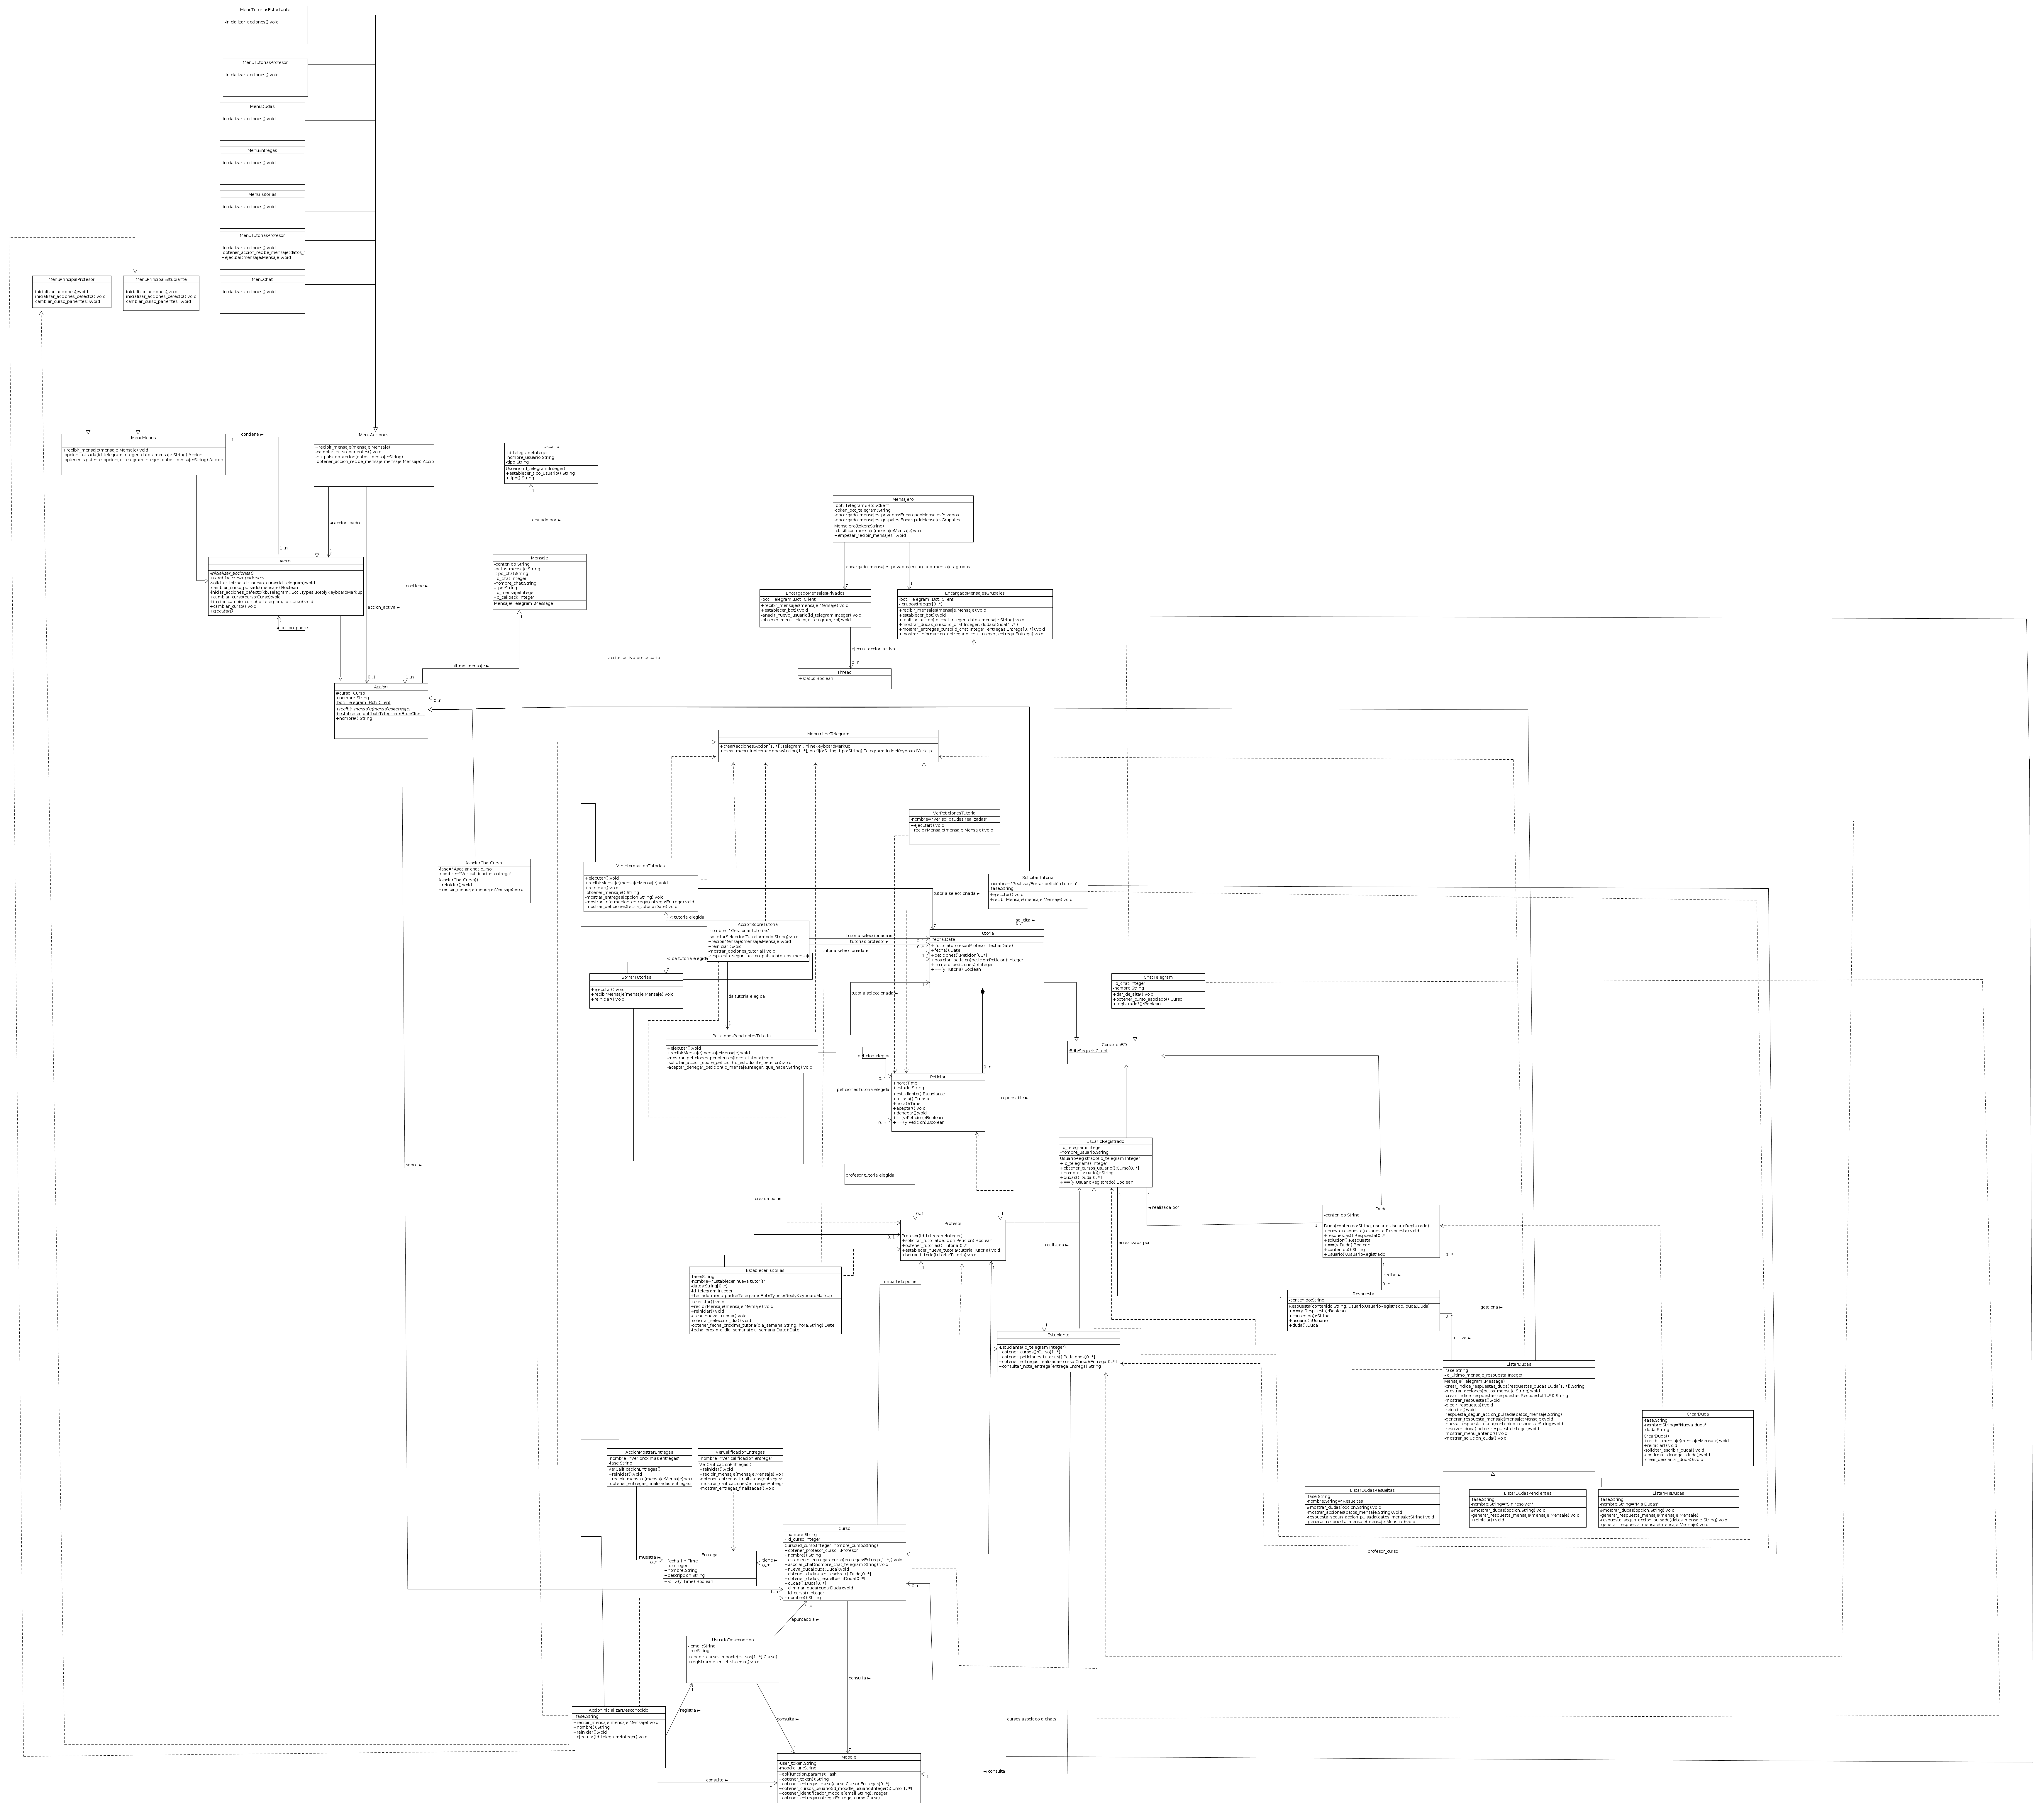
\includegraphics[width=1\textwidth, right]{imagenes/diagramas/diagrama_clases.png}  %el parámetro scale permite agrandar o achicar la imagen. En el nombre de archivo puede especificar directorios
\caption{Diagrama de clases del sistema}\label{figura10101}
\end{figure}
\subsection{Diseño de la configuración de Moodle}

Moodle, como bien se mecionaba en la introducción, proporciona una API accesible a través de lo que ellos llaman \textit{web services}  que permiten especificar las funciones que se pueden llamar de la API y por parte de qué usuarios en qué contexto. A los usuarios se le asigna un rol que es al que se le autoriza a usar un protocolo para comunicarse con los \textit{web services}, siendo también necesario autorizar individualmente a cada usario a que usen un \textit{web service}.  Los protocolos soportados son SOAP, REST o XML-RPC, nosotros vamos a utilizar REST por ser el más sencillo de manejar.
\par

Para el diseño de la configuración de Moodle hay que tener en cuenta lo que necesita el \textit{bot} de Moodle:
\begin{enumerate} 
\item \textit{Bot} necesita que Moodle verifique que los datos que introduce el usuario al registrarse son correctos.
\item \textit{Bot} necesita saber si el usuario que se da de alta es un profesor o un estudiante para darle acceso a una parte u otra de acciones.
\item Tiene que conocer los cursos en los que está matriculado un profesor para que cuando éste se dé de alta, poder registrar estos cursos como usables en el \textit{bot} y, al menos, también tiene que poder saber a qué cursos registrados en el \textit{bot} tiene acceso un estudiante en Moodle.
\item Necesita tener acceso a las entregas abiertas para los cursos que tiene registrados así como a datos como su fecha y si un estudiante lo solicita, a la nota de este estudiante.

\end{enumerate}

Para conseguir configurar Moodle de forma que el \textit{bot} pueda realizar los puntos descritos arriba y que el uso del mismo implique los menos privilegios posibles para evitar cualquier problema con la seguridad y el funcionamiento de la instancia de Moodle, he optado por un enfoque en el cual se empieza con ningún permiso e ir dando poco a poco hasta llegar a lo mínimo necesario.
\par
Los pasos que he seguido son los siguientes:
\begin{enumerate}
\item \textbf{Habilitar los webservices}, para lo cual hay que irse al apartado de \enquote*{Plugins} dentro de \enquote*{Site Administration} buscar \enquote*{Web services} y darle a habilitar.

\item \textbf{Habilitar el protocolo a utilizar}: dentro de Web services buscamos \enquote{Manage protocols} y habilitamos REST.
\begin{figure}[H] %con el [H] le obligamos a situar aquí la figura
\centering
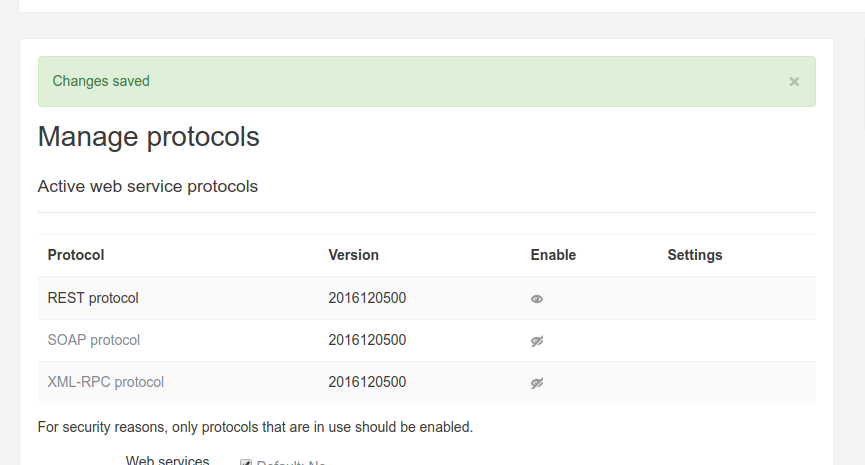
\includegraphics[scale=0.5]{imagenes/moodle/Screenshot_2017-08-25_10-28-32.png}  %el parámetro scale permite agrandar o achicar la imagen. En el nombre de archivo puede especificar directorios

\caption{Habilitando protocolo REST en Moodle}\label{figura410}
\end{figure}
\item Crear tres roles con contexto de sistema con los siguientes permisos mínimos:


\begin{tabular}{|p{5cm}|p{8cm}|}
\hline
\textbf{Nombre rol}
\newline

 &
 
\textbf{Permisos}
  \\
webservices\_bot
\newline

 &
 
\begin{itemize}
\item moodle/course:viewparticipants
\item moodle/user:viewdetails
\item moodle/user:viewhiddendetails
\item moodle/course:useremail
\item moodle/user:update

\end{itemize}
  \\
webservices\_estudiante
\newline

 &
 
\begin{itemize}
\item mod/assign:view
\end{itemize}
  \\
webservice\_profesor
\newline

 &
 

  \\
  \hline
\end{tabular}


\begin{figure}[H] %con el [H] le obligamos a situar aquí la figura
\centering
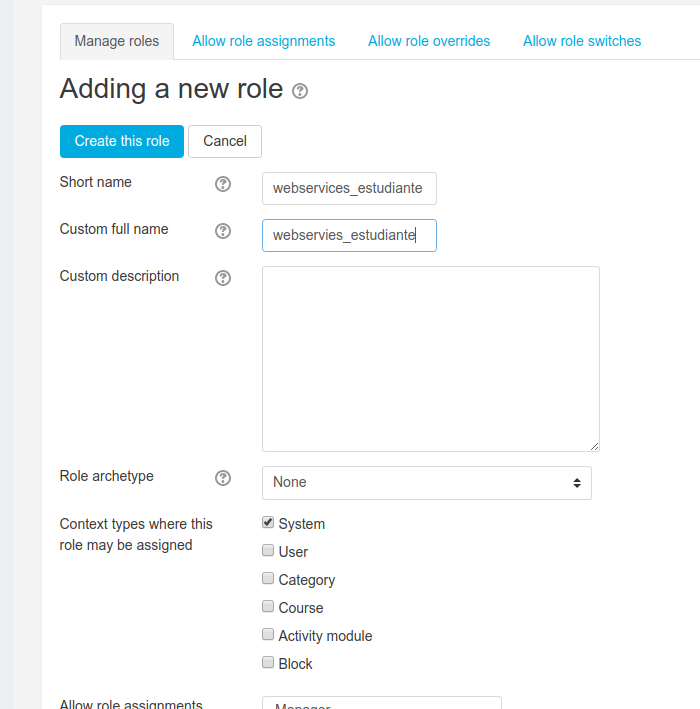
\includegraphics[scale=0.4]{imagenes/moodle/Screenshot_2017-08-25_11-11-23.png}  %el parámetro scale permite agrandar o achicar la imagen. En el nombre de archivo puede especificar directorios

\caption{Creando rol webservices\_student}\label{figura412}
\end{figure}

Estos permisos son los imprescindibles para poder utilizar las funciones descritas en la siguiente tabla. Si no fueran roles con contexto de sistema entonces no tendrían acceso a los \textit{web servies}.

\item Crear los siguientes webservices marcando \enquote*{enable} y \enquote*{Authorized users only}   con las siguientes funciones cada uno:

\begin{tabular}{|p{5cm}|p{8cm}|}
\hline
\textbf{Webservice}
\newline

 &
 
\textbf{Funciones}
  \\
webservices\_bot
\newline

 &
 
\begin{itemize}
\item \textbf{core\_enrol\_get\_users\_courses}: Permite al bot obtener los cursos de un usuario cuando éste se identifica ante el bot por primera vez.
\item \textbf{core\_user\_get\_users\_by\_field}: Permite obtener el identificador de moodle del usuario recién registrado, necesario para conocer las notas de su entrega.
\item \textbf{mod\_assign\_get\_assignments}: Permite al bot obtener las entregas abiertas para un curso junto con detalles como su fecha.
\end{itemize}
  \\
webservices\_estudiante
\newline

 &
 
\begin{itemize}
\item \textbf{mod\_assign\_get\_assignments}: Permite al estudiante ver las entregas para los cursos a los cuales tiene acceso.
\item \textbf{mod\_assign\_get\_submission\_status}: Un estudiante puede con su token, id de moodle e id entrega puede ver que calificación tiene en la entrega.
\end{itemize}
  \\
webservice\_profesor
\newline

 &
 

  \\
  \hline
\end{tabular}

\begin{figure}[H] %con el [H] le obligamos a situar aquí la figura
\centering
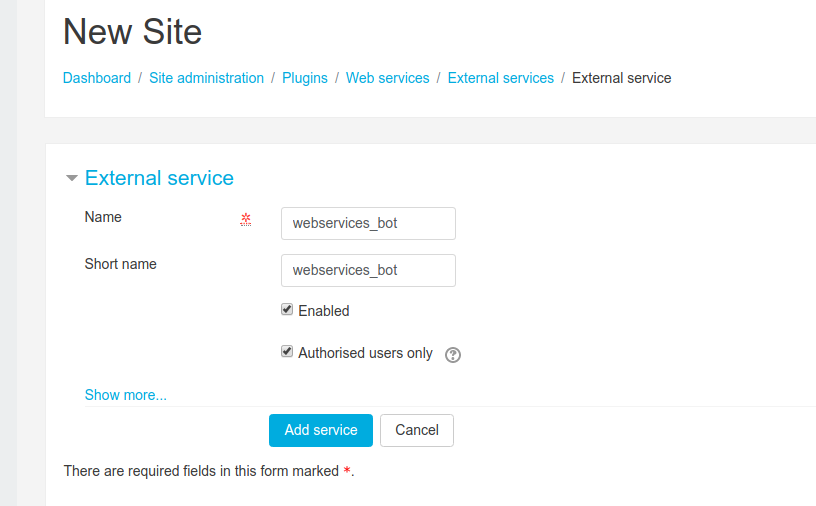
\includegraphics[scale=0.5]{imagenes/moodle/Screenshot_2017-08-25_11-24-11.png}  %el parámetro scale permite agrandar o achicar la imagen. En el nombre de archivo puede especificar directorios

\caption{Creando webservice llamado webservices\_bot}\label{figura415}
\end{figure}

\begin{figure}[H] %con el [H] le obligamos a situar aquí la figura
\centering
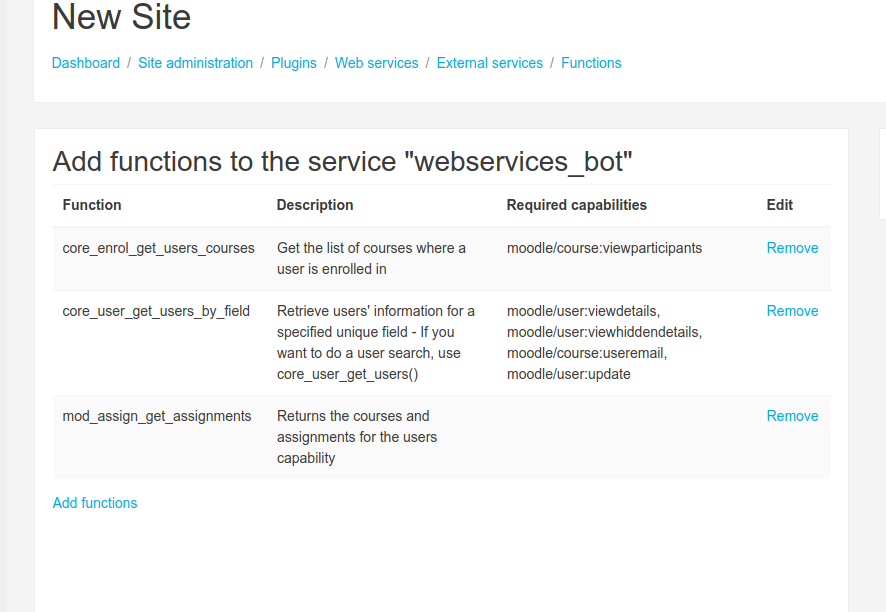
\includegraphics[scale=0.3]{imagenes/moodle/Screenshot_2017-08-25_11-27-44.png}  %el parámetro scale permite agrandar o achicar la imagen. En el nombre de archivo puede especificar directorios

\caption{Añadiendo funciones a el webservice llamado webservices\_bot }\label{figura415}
\end{figure}



\item Crear un usuario en Moodle para el bot.
\item Asignar el rol de webservices\_estudiante a los usuarios de moodle que quieren utilizar el bot como estudiantes, el webservices\_profesor a los profesores y el webservice\_bot al usuario que se ha creado para el bot. Como son roles de sistema es necesario irse al apartado \texttt{Site Administration > Users > Assign system roles services}:

\begin{figure}[H] %con el [H] le obligamos a situar aquí la figura
\centering
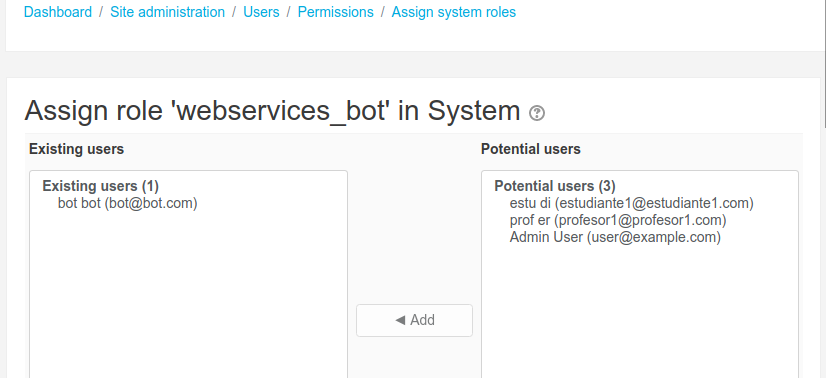
\includegraphics[scale=0.3]{imagenes/moodle/Screenshot_2017-08-25_14-40-20.png}  %el parámetro scale permite agrandar o achicar la imagen. En el nombre de archivo puede especificar directorios

\caption{Asignado el rol webservices\_bot al usuario creado en Moodle para el bot }\label{figura418}
\end{figure}

\item Añadir a los usuarios a los que se les ha asignado como rol webservices\_estudiante como usuarios autorizados a usar el recien creado webservices\_estudiante, a los que tienen rol webservices\_profesor añadir como usuarios autorizados al webservice webservices\_profesor y al usuario del bot con rol webservices\_bot añadirlo como usuario autorizado webservice\_bot. 

\begin{figure}[H] %con el [H] le obligamos a situar aquí la figura
\centering
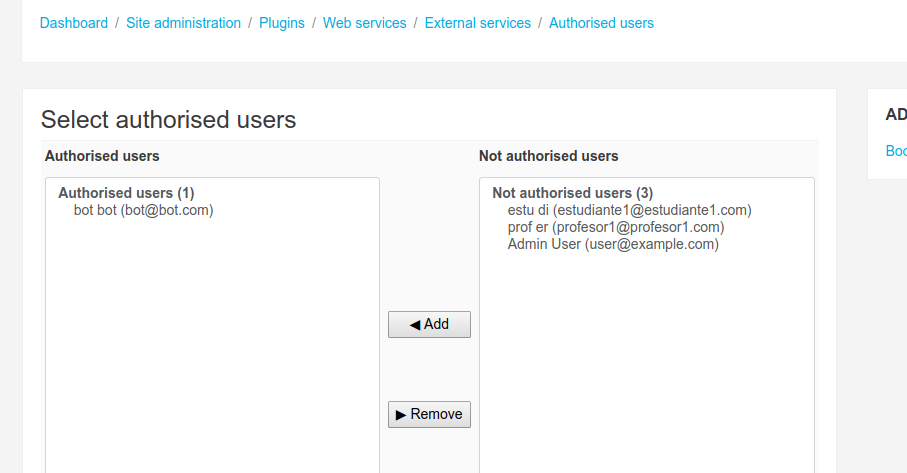
\includegraphics[scale=0.3]{imagenes/moodle/Screenshot_2017-08-25_11-48-23}  %el parámetro scale permite agrandar o achicar la imagen. En el nombre de archivo puede especificar directorios

\caption{Asignado el rol webservices\_bot al usuario creado en Moodle para el bot }\label{figura419}
\end{figure}

\item Crear token para el usuario que se ha creado en Moodle para el bot. Esto se puede hacer bajo el apartado Web services buscando \texttt{Manage tokens}.



\begin{figure}[H] %con el [H] le obligamos a situar aquí la figura
\centering
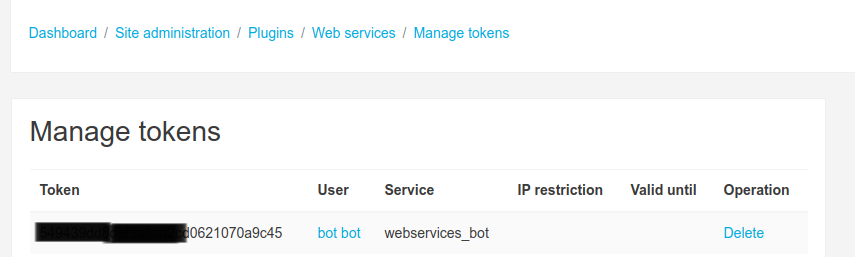
\includegraphics[scale=0.3]{imagenes/moodle/Screenshot_2017-08-25_11-59-03.png}  %el parámetro scale permite agrandar o achicar la imagen. En el nombre de archivo puede especificar directorios

\caption{Creando token para el usuario en Moodle del bot }\label{figura419}
\end{figure}
\item Añadir en Moodle al usuario creado para el bot a cada curso que se quiera que tenga acceso el bot.

\begin{figure}[H] %con el [H] le obligamos a situar aquí la figura
\centering
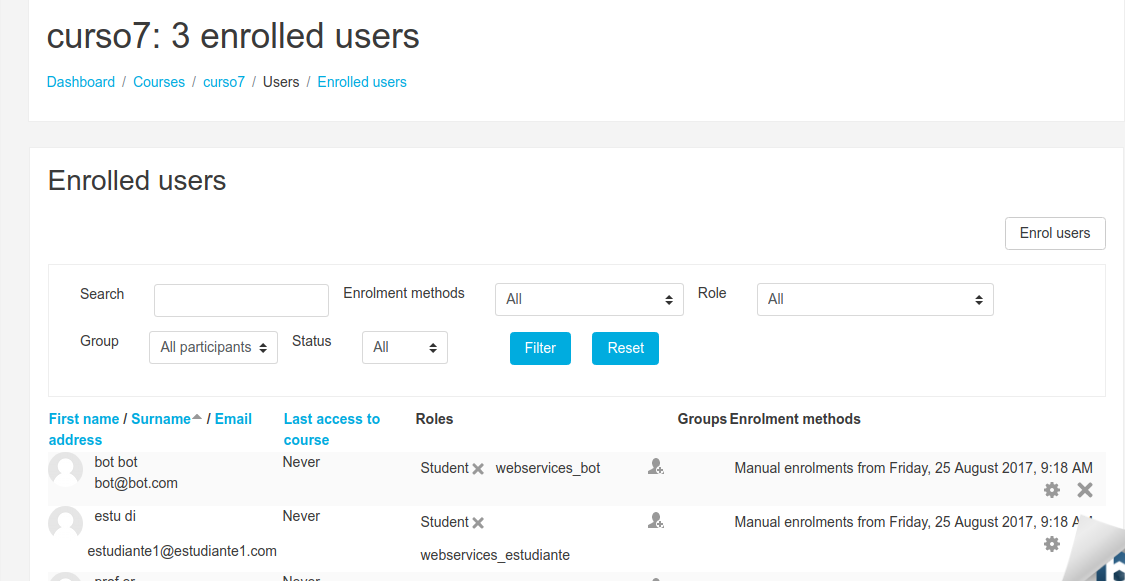
\includegraphics[scale=0.3]{imagenes/moodle/Screenshot_2017-08-25_12-19-29.png}  %el parámetro scale permite agrandar o achicar la imagen. En el nombre de archivo puede especificar directorios

\caption{Añadiendo al usuario bot al curso curso7 }\label{figura420}
\end{figure}
\end{enumerate}



Una vez hecho esto podemos comprobar si tenemos acceso a las funciones de los \textit{web services} a traves de REST utilizando un navegador web:
\begin{figure}[H] %con el [H] le obligamos a situar aquí la figura
\centering
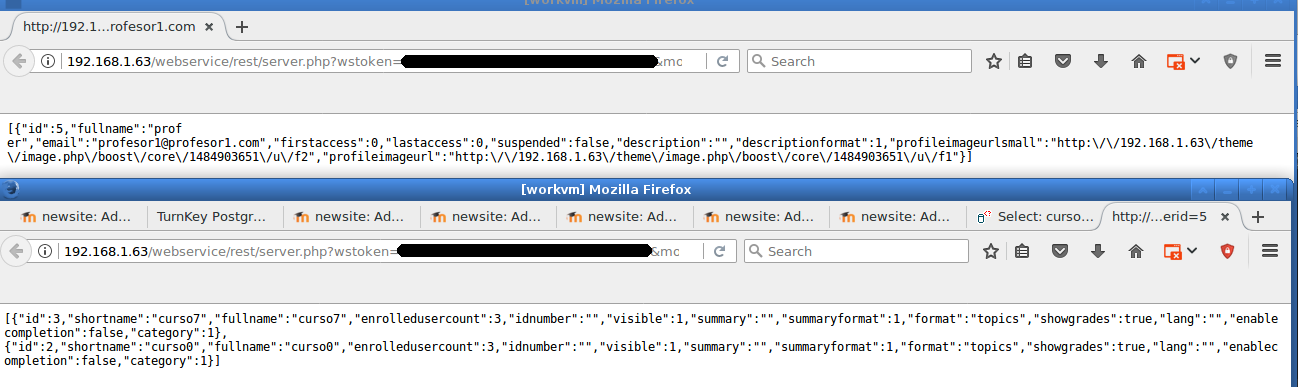
\includegraphics[scale=0.35]{imagenes/moodle/Screenshot_2017-08-25_12-32-18.png}  %el parámetro scale permite agrandar o achicar la imagen. En el nombre de archivo puede especificar directorios

\caption{Llamando a algunas de las funciones de webservices\_bot a través del navegador web }\label{figura420}
\end{figure}

Todo el proceso anteriomente descrito se puede encontrar en la sección \texttt{ Site Administration > Plugins > Web services} de cualquier instancia de Moodle.

\subsubsection{Justificación}

Se han creado tres \textit{web services} con tres roles diferentes ya que hay tres tipos de usuarios y cada uno necesita acceder a un conjunto de funciones diferentes. Si tuviéramos un solo rol y un solo \textit{web service} entonces algunos usuarios tendrían más permisos de los necesarios y acceso a funciones de la API que no les hacen falta.
\par
Ejemplo: al \textit{bot} no le hace falta hacer llamadas a la función que obtiene calificaciones de la entrega y por tanto mejor no darle acceso. 
\par
Cada usuario del sistema en el momento que introduce sus datos de Moodle para empezar a usar el bot éste obtiene una token de usuario y con esa token el usuario solamente tiene acceso a su información individual (caso de los estudiante que cuando llaman a \texttt{mod\_assign\_get\_submission\_status} les devuelve datos de las entregas del usuario cuya token se utiliza para llamar al \textit{web service}.)
\par
Hace falta un token aparte para el \textit{bot} porque éste necesita conocer información común de un curso como las entregas que hay abiertas, si no tiene token entonces no hay acceso. Además si no creáramos un usuario aparte para el \textit{bot} entonces no se puede controlar a qué cursos tienen acceso los usuarios del \textit{bot}. Obligando a añadir al bot a un curso de Moodle hacemos que los usuarios que soliciten al bot usarlo solamente tengan acceso a aquellos cursos en los que el bot ha sido añadido. Esto es importante ya que dando rol con contexto de sistema a un usuario hacemos que tenga acceso con su token a todos los cursos en los que están matriculados en Moodle (limitado a las funciones permitidas en su webservice y a los permisos de su rol) tanto si el profesor responsable de ese curso quiere o no quiere utilizar los webservices de Moodle para ese curso.

\newpage
\subsection{Diseño de la base de datos}

La estructura lógica de la base de datos se puede observar en el siguiente diagrama ER:

\begin{figure}[H] %con el [H] le obligamos a situar aquí la figura
\centering
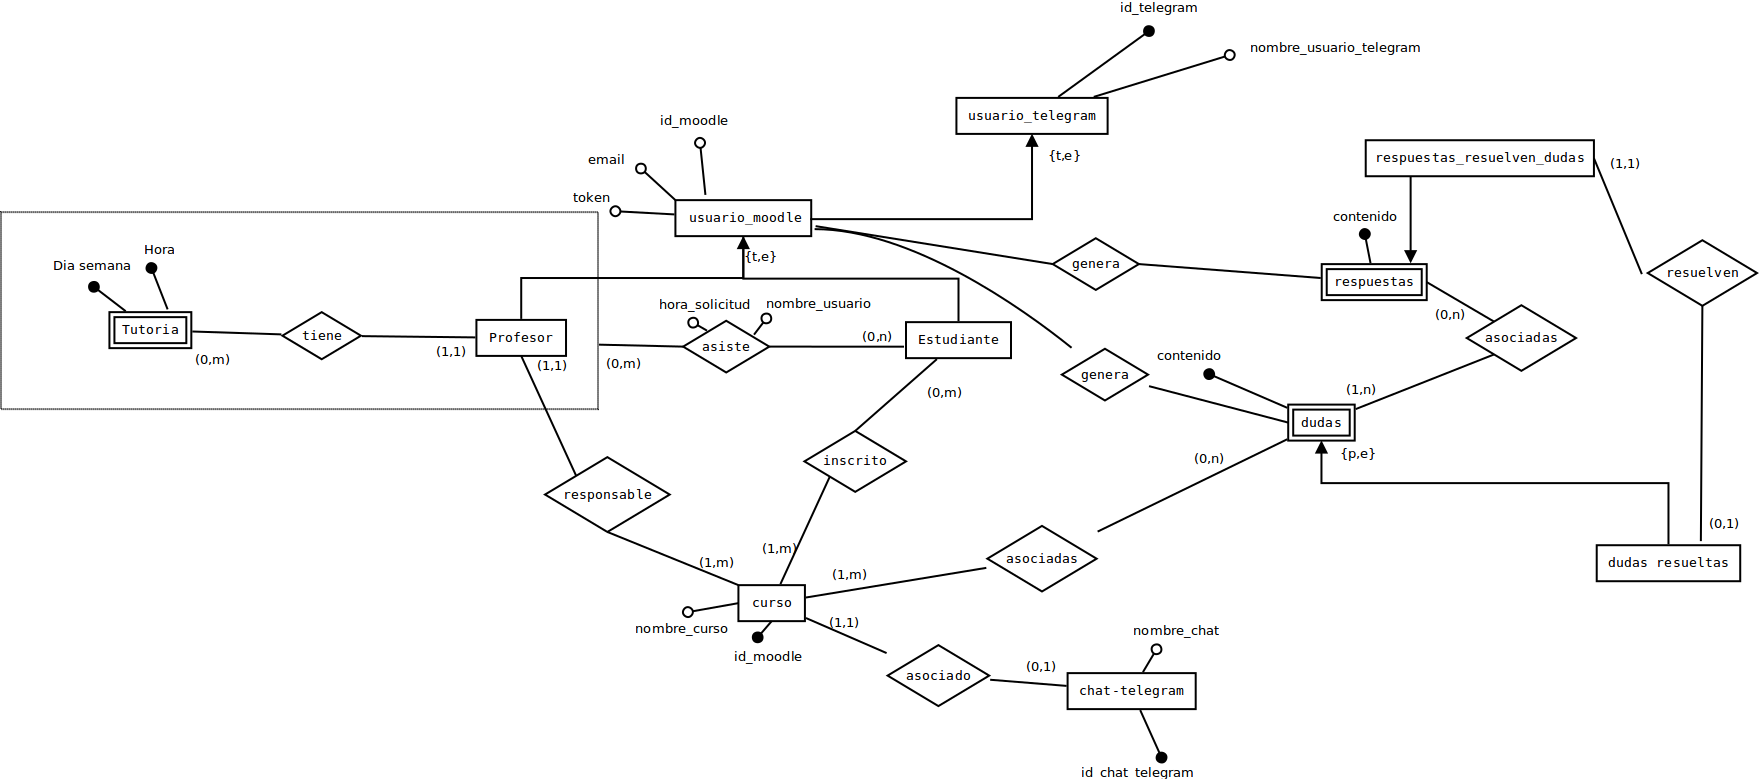
\includegraphics[scale=0.2]{imagenes/diagramas/base_datos/ER.png}  %el parámetro scale permite agrandar o achicar la imagen. En el nombre de archivo puede especificar directorios

\caption{Diagrama ER de la base de datos }\label{figura520}
\end{figure}
Se pueden apreciar las necesidades de almacenamiento que va a tener nuestra aplicación y podemos extraer el esqueleto de la base de datos con sus relaciones, claves externas, primarias... \par
Tras realizar el paso a tablas de este diagrama y efectuar el paso a la tercera forma normal obtenemos el siguiente esquema de la base de datos:


 \begin{figure}[H] %con el [H] le obligamos a situar aquí la figura
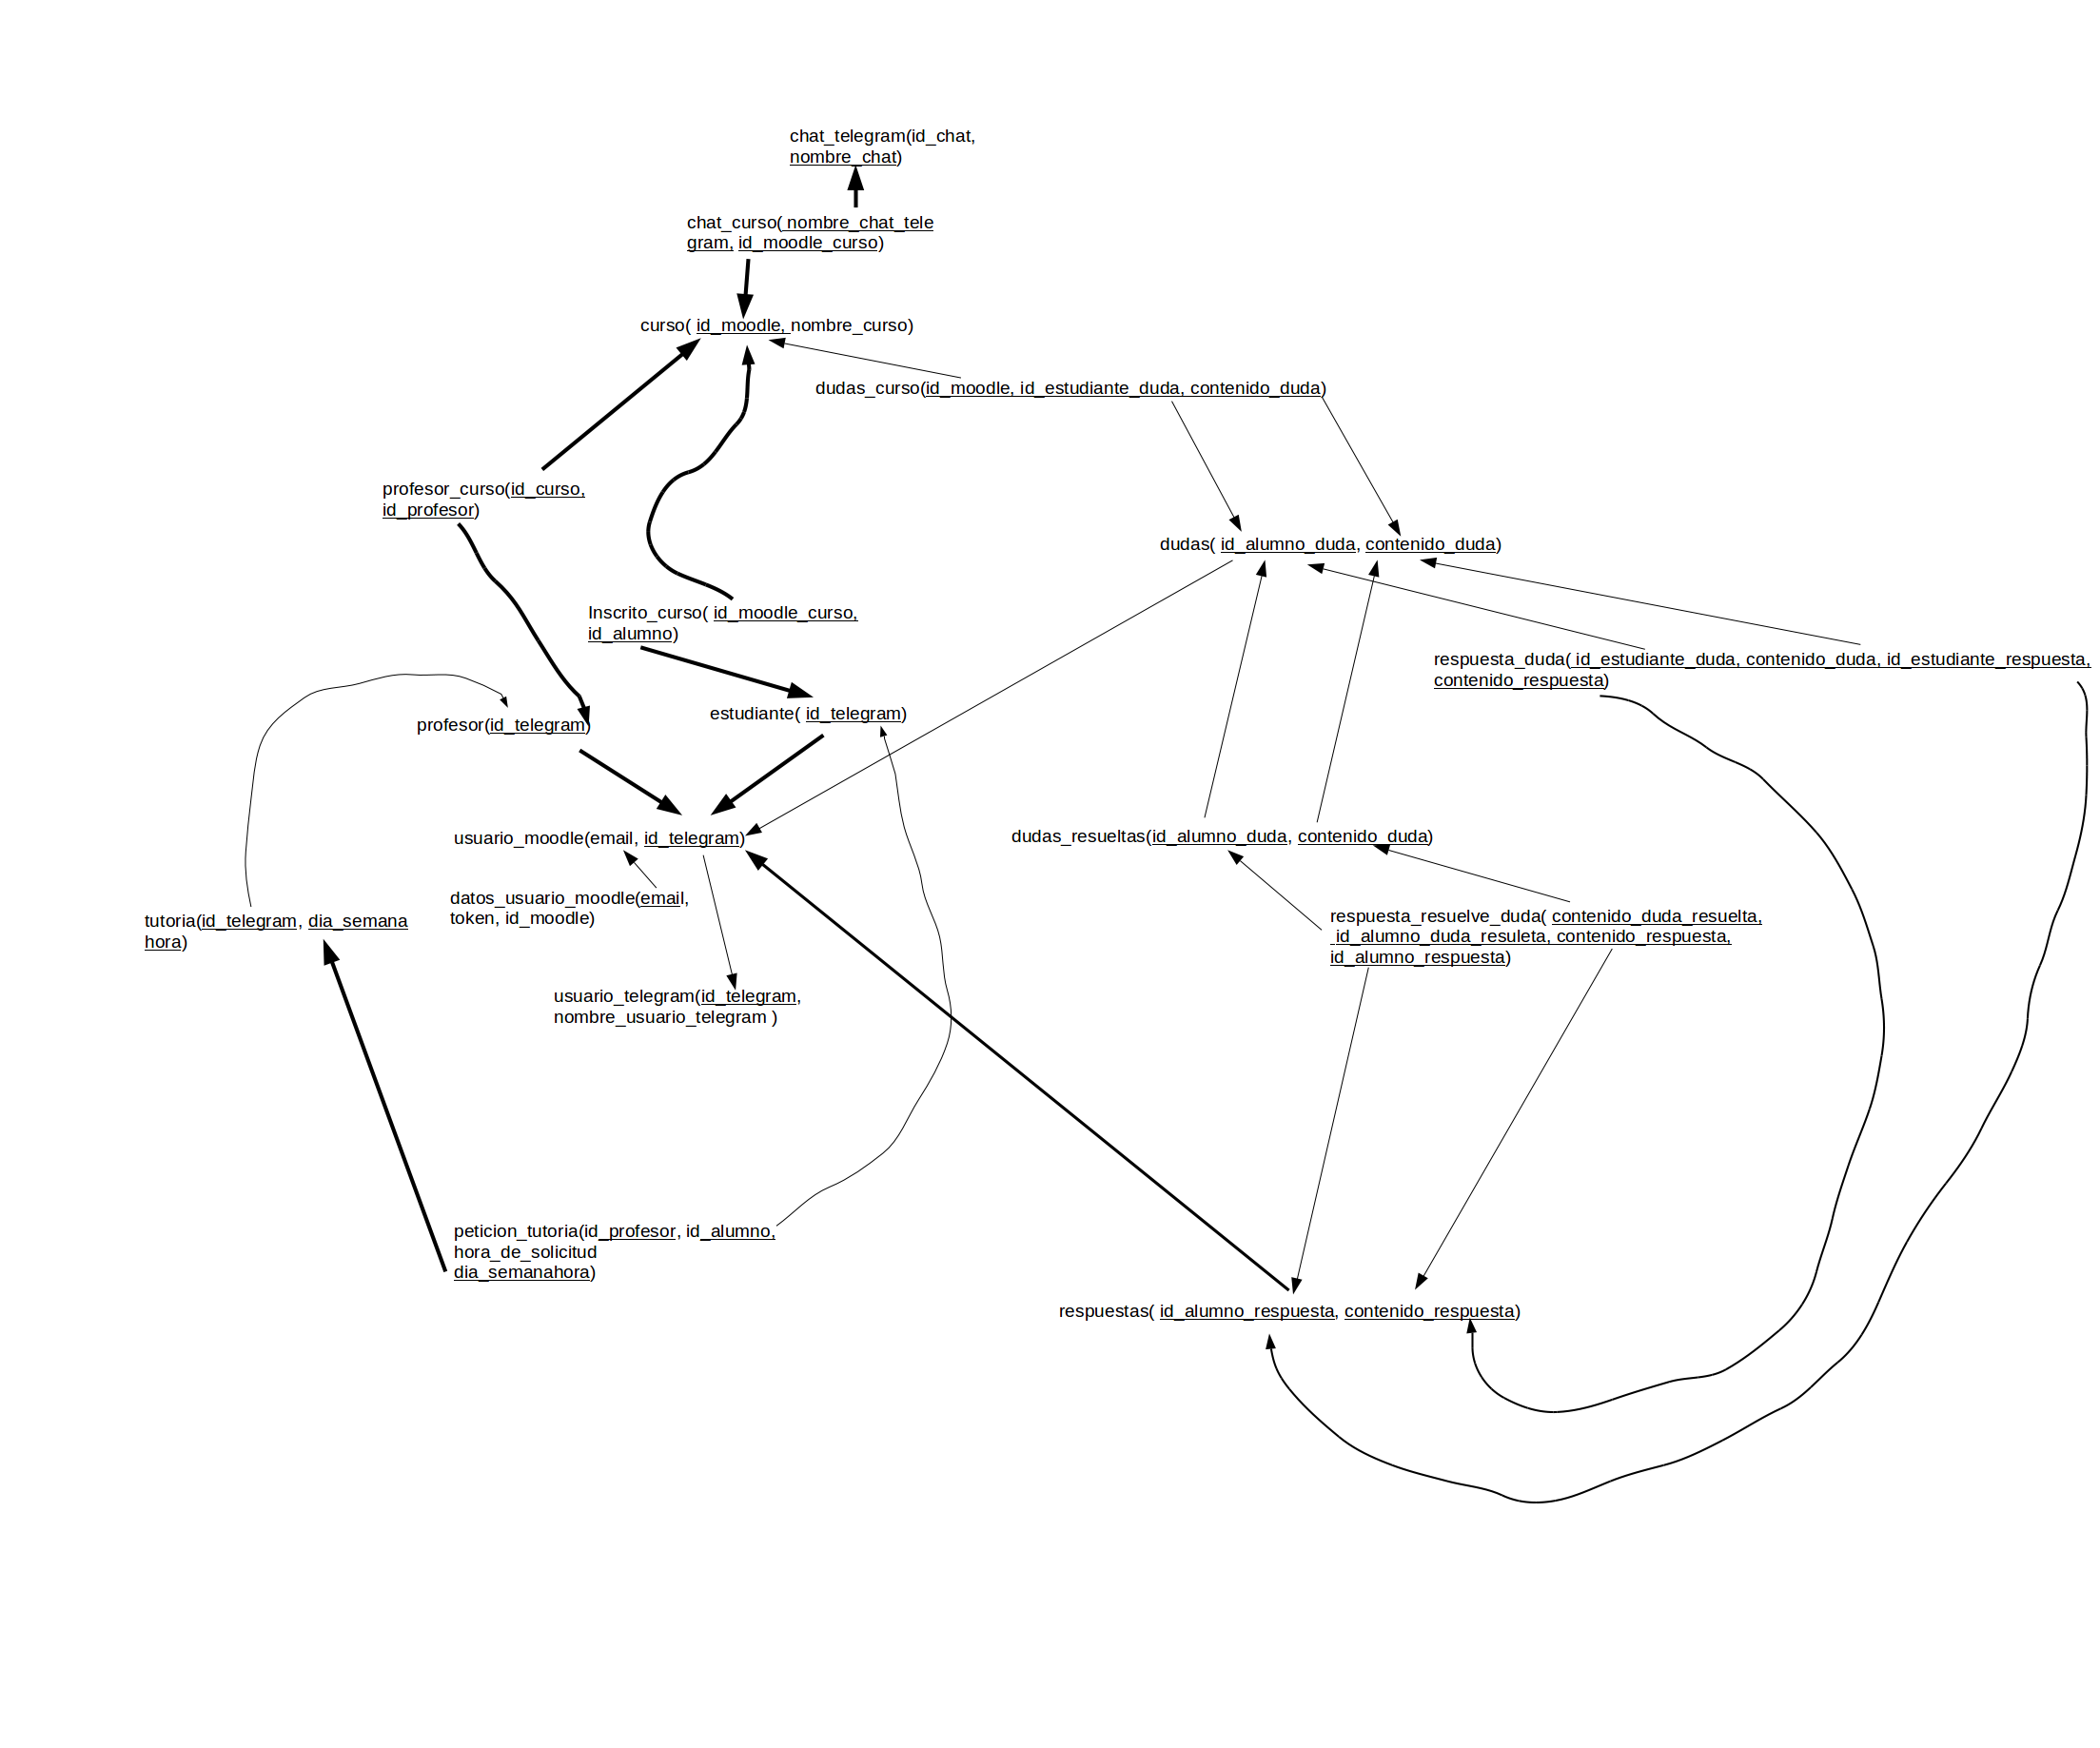
\includegraphics[width=1.2\textwidth, right]{imagenes/diagramas/base_datos/esquema_tablas_normalizadafn3.png}  %el parámetro scale permite agrandar o achicar la imagen. En el nombre de archivo puede especificar directorios
\caption{Esquema base datos en tercera forma normal}\label{figura5211}
\end{figure}



\subsection{Diseño de los tests}

En el desarrollo de la aplicación se está siguiendo la programación orientada a objetos como paradigma de programación. Para verificar el correcto funcionamiento de las clases que la componen se hace uso de test unitarios que prueban la \enquote*{interfaz} o parte pública de la clase proporcionándole datos de prueba y comprobando si los resultados devueltos por ésta son los esperados.
\par
A la hora de diseñar estos tests unitarios hay que tener en cuenta que básicamente hay dos tipos de clases: aquellas que reciben un mensaje y realizan algo con este (bien sea extraer los datos de éste y realizar una acción o entregar el mensaje a la clase responsable) y las que acceden a la base de datos y Moodle. Para los tests de las primeras se hará uso de stubs para simular clases con una serie de métodos predefinidos que devuelven datos ideales y  de mocks para monitorizar si la clase bajo prueba realiza las acciones deseadas cuando se le entrega un mensaje con unas características predeterminadas.\\
Para las segundas debido a la dificultad de simular una base de datos se optará por crear una base de datos \enquote*{desechable} en la cual se introducen una serie de datos prefijados y se prueba el comportamiento de la interfaz pública de estas clases, bien llamando a sus métodos públicos y comprobando el resultado devuelto, o bien comprobando el efecto sobre la base de datos.
